\section{Simulation results}\label{secExpRes}
In this section simulation results of the application of the proposed approach to SDN Priority Queueing identification and control will be provided. Standard RFs are used to derive predictive models of the disturbance components $d_1(k),\ldots,d_8(k)$, i.e. the switch input differentiated for each DSCP index, and validate the accuracy. Then the validation of accuracy of the predictive model of the output variable $y(k)$ derived as illustrated in Section \ref{secSwitchedModeling} is shown: the predictive models (based on RTs and RFs) will be compared with Artificial Neural Networks, showing that RFs represent the ideal solution both in terms of prediction accuracy and computational complexity; then it will be illustrated the effect of iterative dataset updates in the prediction accuracy, both with and without prediction of the future disturbances. Finally it will be used the proposed predictive models to setup a MPC problem (see Problem \ref{pbMPC}), and validate the control performance in terms of packet losses reduction and bandwidth saving, both with and without prediction of the future disturbances. It will also be shown, as expected, that using accurate predictive models and applying MPC provides dramatic reduction of packet losses and increase of bandwidth saving with respect to the static bandwidth allocation policy used in Service Provider Networks as described in Section \ref{sec:SDNNetSim}: even thought this result is not surprising, it is decided to quantify the gap to emphasize that much better performance can be obtained in real networks just collecting historical data and applying a controller that can be directly implemented using the accurate models of the proposed identification algorithm and Quadratic Programming solvers (which are well known to be very efficient).

In each of the aforementioned validations, 4 different predictive models have been exploited, using iteratively enriched data sets. More precisely, \textbf{OLD} is a predictive model identified with a data set of $5124$ samples, collected with a sampling time of $5$ minutes and obtained from network emulation with random values of the input $u(k)$; \textbf{1UP} is a predictive model identified with the \textbf{OLD} data set enriched with $3456$ new samples obtained from network emulation when applying closed-loop MPC to define the input $u(k)$; \textbf{2UP} is a predictive model identified with the \textbf{1UP} data set enriched with $3168$ new samples obtained from network emulation when applying closed-loop MPC to define the input $u(k)$; \textbf{3UP} is a predictive model identified with the \textbf{2UP} data set enriched with $6336$ new samples obtained from network emulation when applying closed-loop MPC to define the input $u(k)$. An independent data-set composed by $1684$ samples is used to validate the above models.
%Before running the identification algorithms, the dataset has been pre-processed checking if all measurements were coherent and if there were voids or data misalignments that could have distorted the model.
All simulations have been ran on a UDOO x86 Advanced with an Intel Braswell N3160 processor up to 2.24 GHz and 4 GB of RAM \cite{UDOO}.

%====================================================================================================

\section {Disturbance predictive model validation} Having an accurate predictive model of the variable $d(k)$ (i.e. the switch input differentiated for each DSCP index) can be helpful to improve the model identification performance as well as the reference input $x_{\mathrm{ref},j} \hspace{3pt} j=1,2, \hdots, N$ to follow in Problem \ref{pbMPC}. In this section  standard RF algorithms are applied, with a regressive index of $15$ steps and $30$ trees for each forest, to obtain a predictive model of the disturbance over a predictive horizon of $N=5$ ($25$ minutes): this choice of $N$ has been taken considering the tradeoff between time complexity of the identification algorithm and the obtained identification accuracy. 

\begin{figure}[h!]
	\centering
	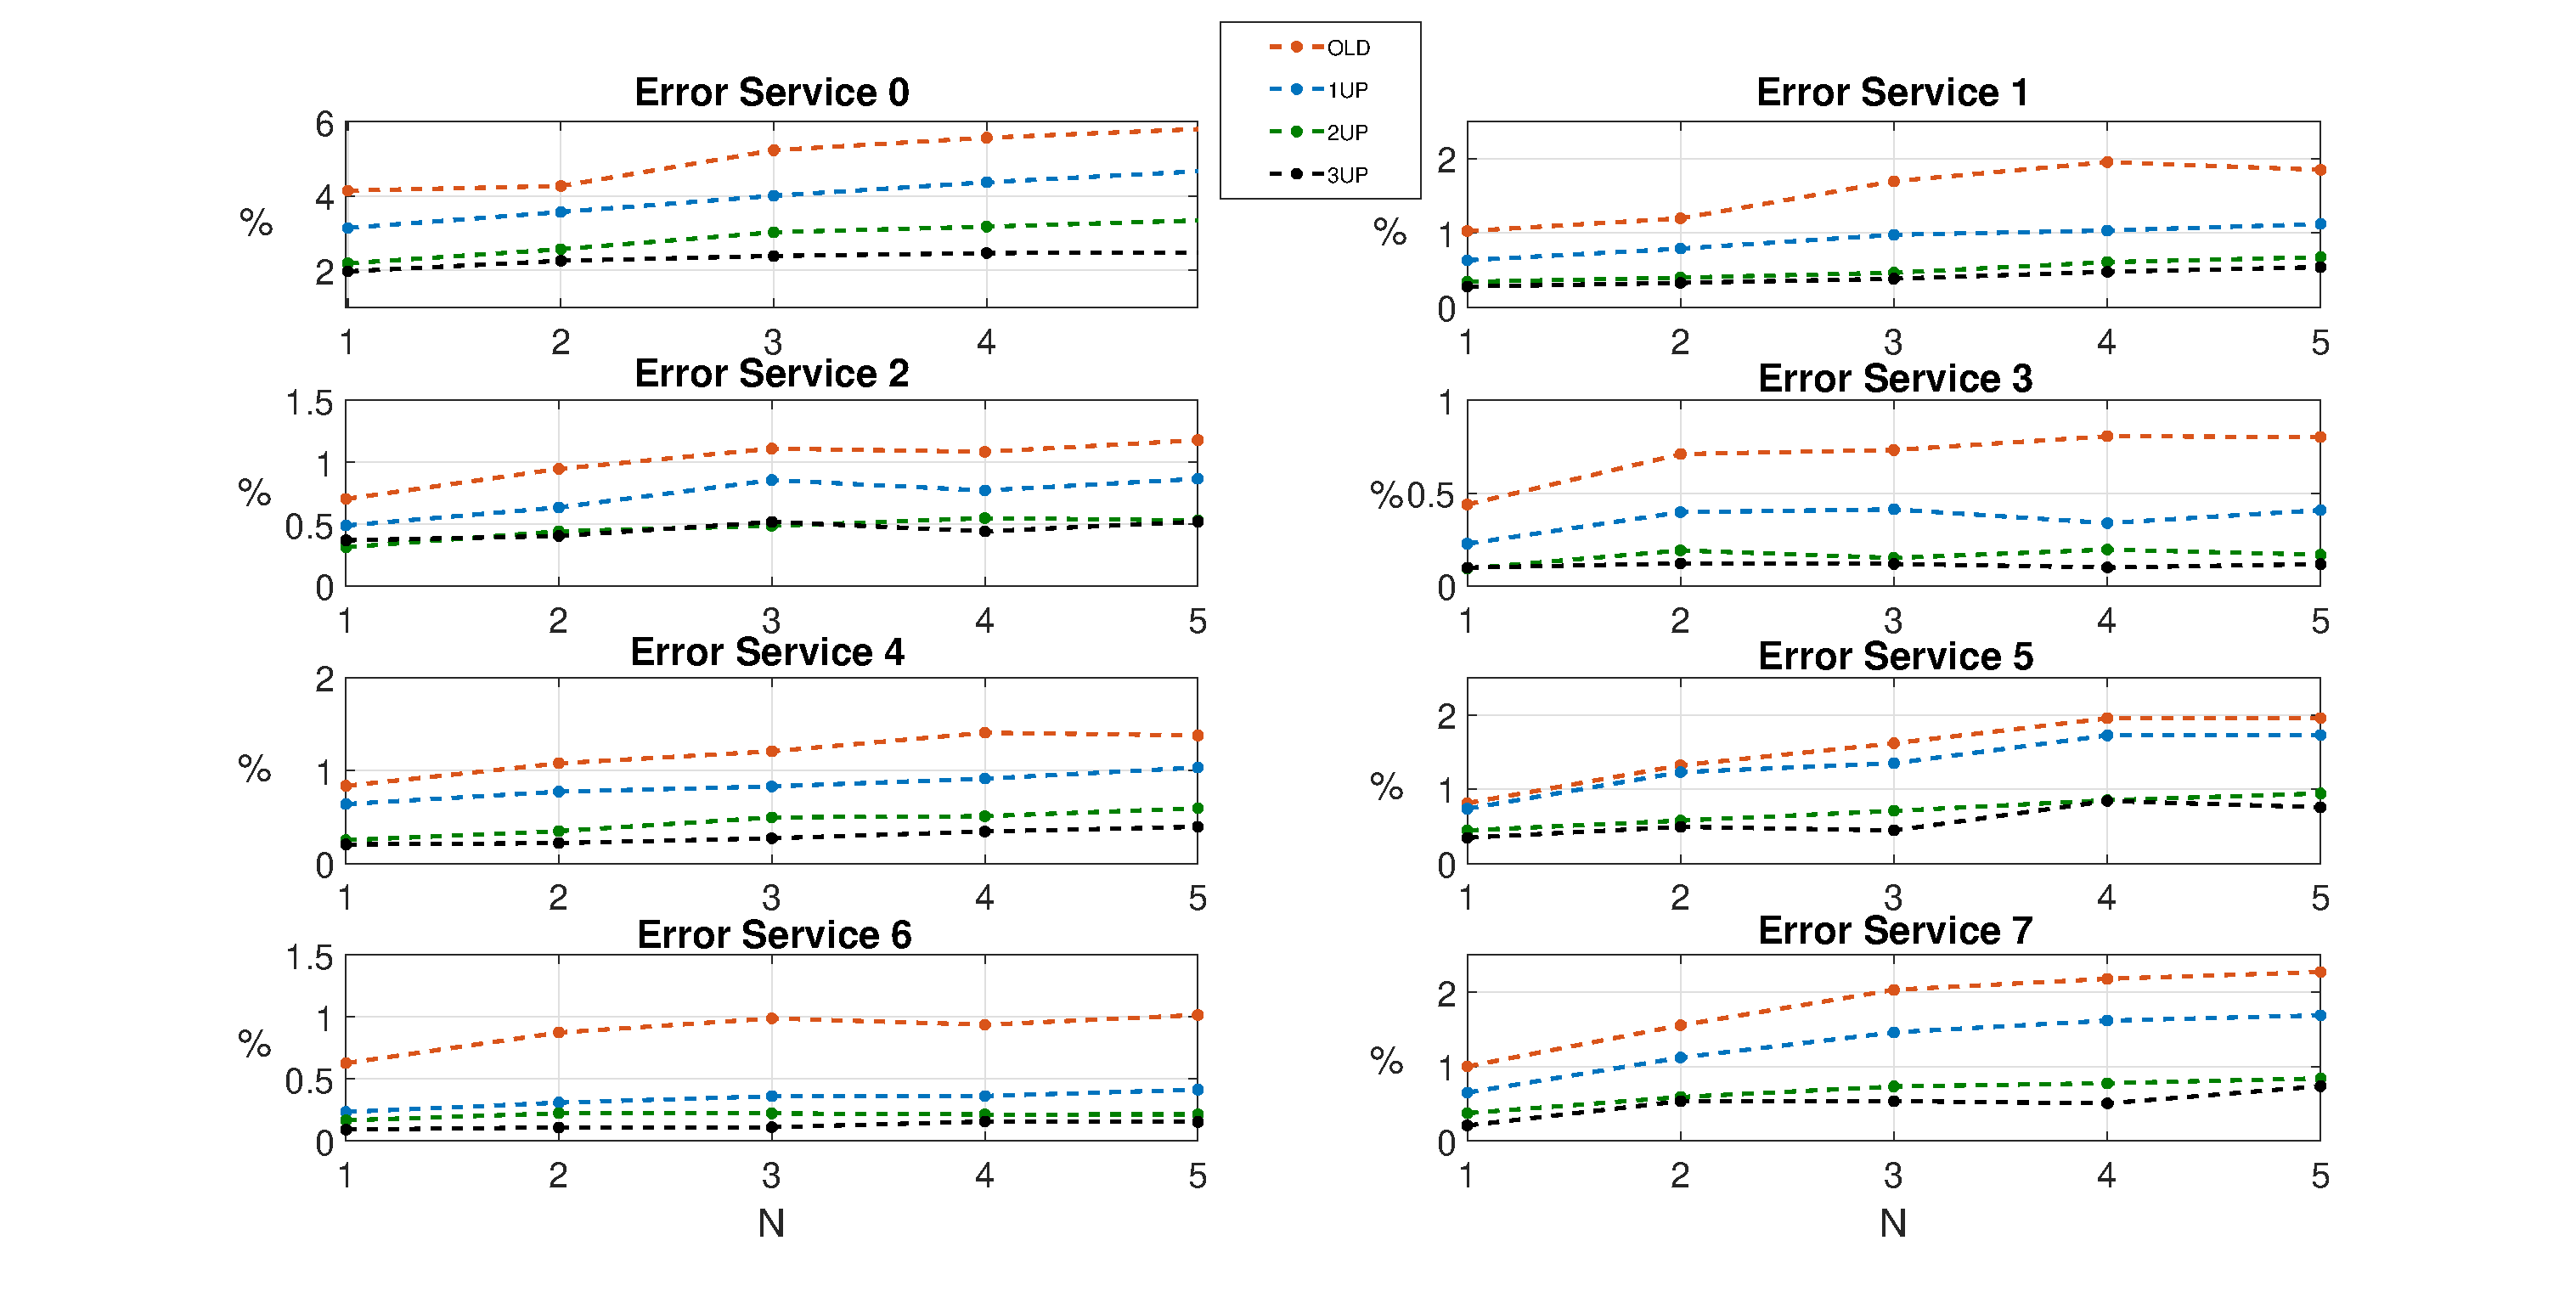
\includegraphics[trim={120 0 120 0}, width=1\linewidth]{figure/Error_Disturbance.eps}
	\caption{NRMSE of the disturbance predictive model over a time horizon of $N=5$.}
	\label{fig:{errorDist}}
\end{figure}
\begin{figure}[h!]
	\centering
	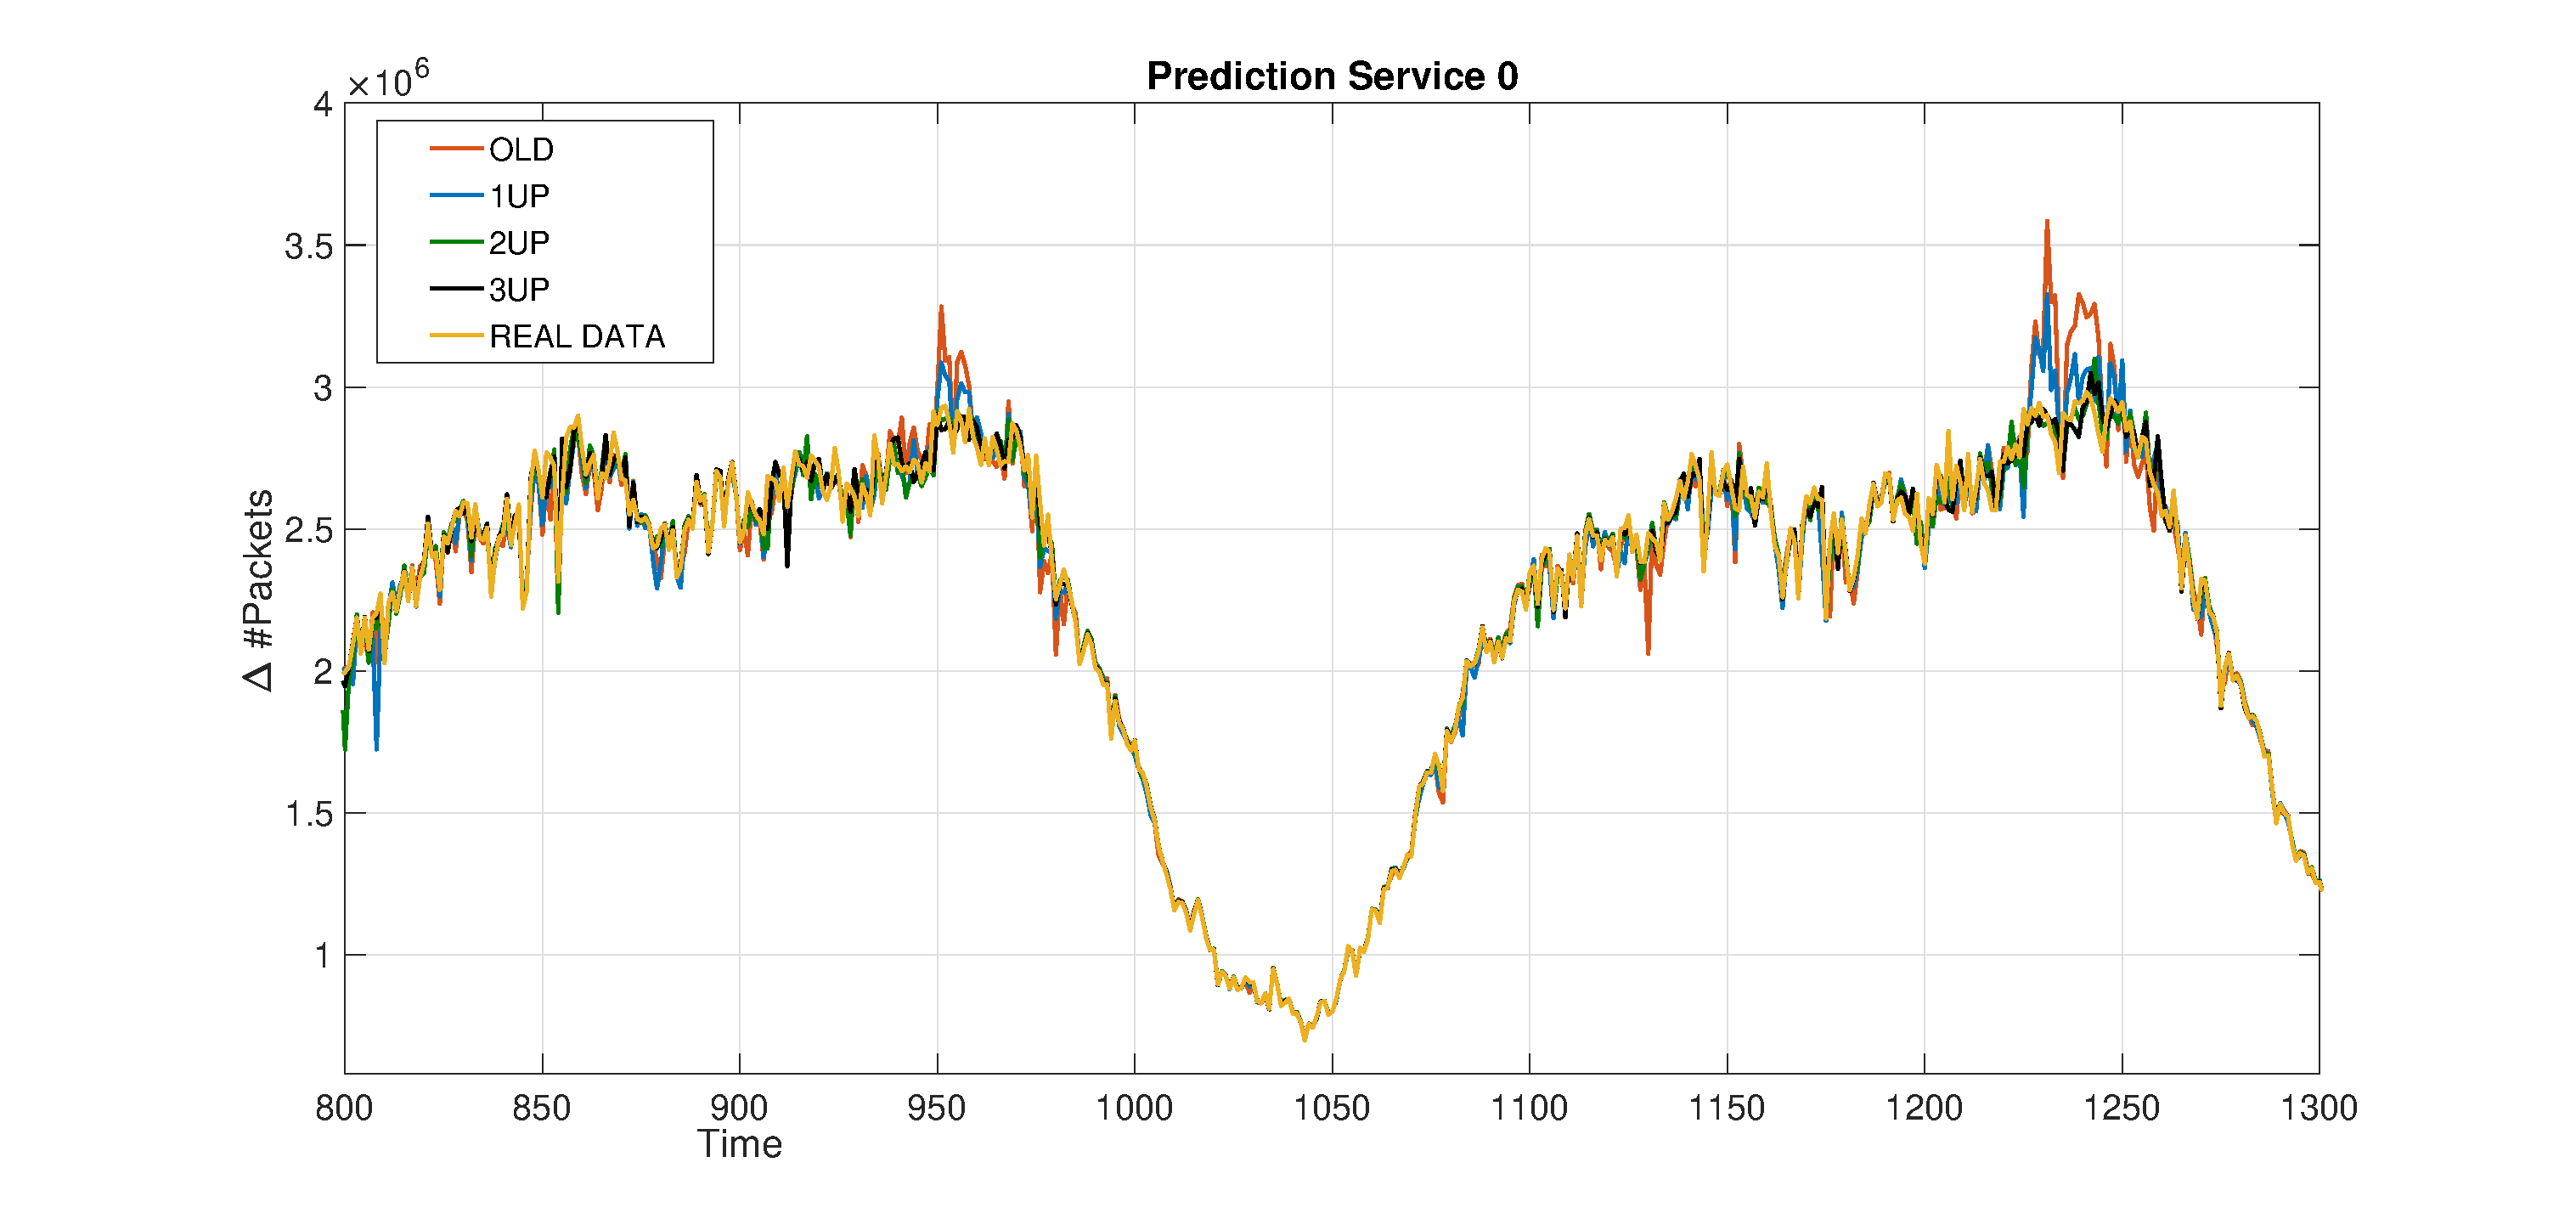
\includegraphics[trim={120 0 120 0}, width=1\linewidth]{figure/Error_Disturbance_Packets.eps}
	\caption{Comparison between the real traffic (YELLOW LINE) and the traffic prediction for the different models for Service 0.}
	\label{fig:{errorPack}}
\end{figure}

Figure \ref{fig:{errorDist}} shows the Normalised Root Mean Square Error (NRMSE) of the predictive model of the disturbance signals (one for each of the 8 DSCP indices) over a time horizon of $N=5$: the prediction error is worse for Service $0$ ($4-6\%$) since it includes the majority of the packets that transit through the switch. For other services the NRMSE is at most $2.2\%$ (Service 7) over all the predictive horizons. The improvement of the model accuracy when using larger (updated) data sets is evident, until a \textit{saturation} is reached and further data do not help to improve the model accuracy: the NRMSE significantly reduces and for Service 0 it is even halved. Figure \ref{fig:{errorPack}} plots, for Service $0$ and in a time window of $500$ samples (almost two days), the predictions of OLD, 1UP, 2UP and 3UP as well as the original data, and clearly highlights the better prediction of 2UP and 3UP with respect to OLD and 1UP.

%====================================================================================================
\subsection{Traffic predictive model validation on real network data}

{In addition to the validation of our predictive models of the incoming traffic over the Mininet environment, the accuracy has been also tested on data measured from a real network device (Ubiquiti EP-16) of an Italian internet internet provider (Sonicatel S.r.l.). Data collection has been performed using the software Cacti \cite{Cacti}.\\
Since this device is part of a running commercial network, some constraints in data collection have forced to only measure the sum of all packets entering and leaving the device, and it has been possible to extract from such traffic only incoming VOIP packets: i.e., it has not been possible to extract packets differentiated for each DSCP. Moreover, it is not currently possible to apply any type of closed-loop control on the network device. For the above 2 reasons the control performance validation in the following sections is not based on this real traffic dataset.\\
About data analysis, 53 days of data measurements have been used for RF training and about 3 days for model validation. Figure \ref{fig:{errorPescara}} shows the prediction on three classes of packets: all packets received, all packets transmitted, VOIP packets received. The plots show that our methodology provides a very accurate prediction even on a real internet service provider network.}
\begin{figure}[h!]
	\centering
	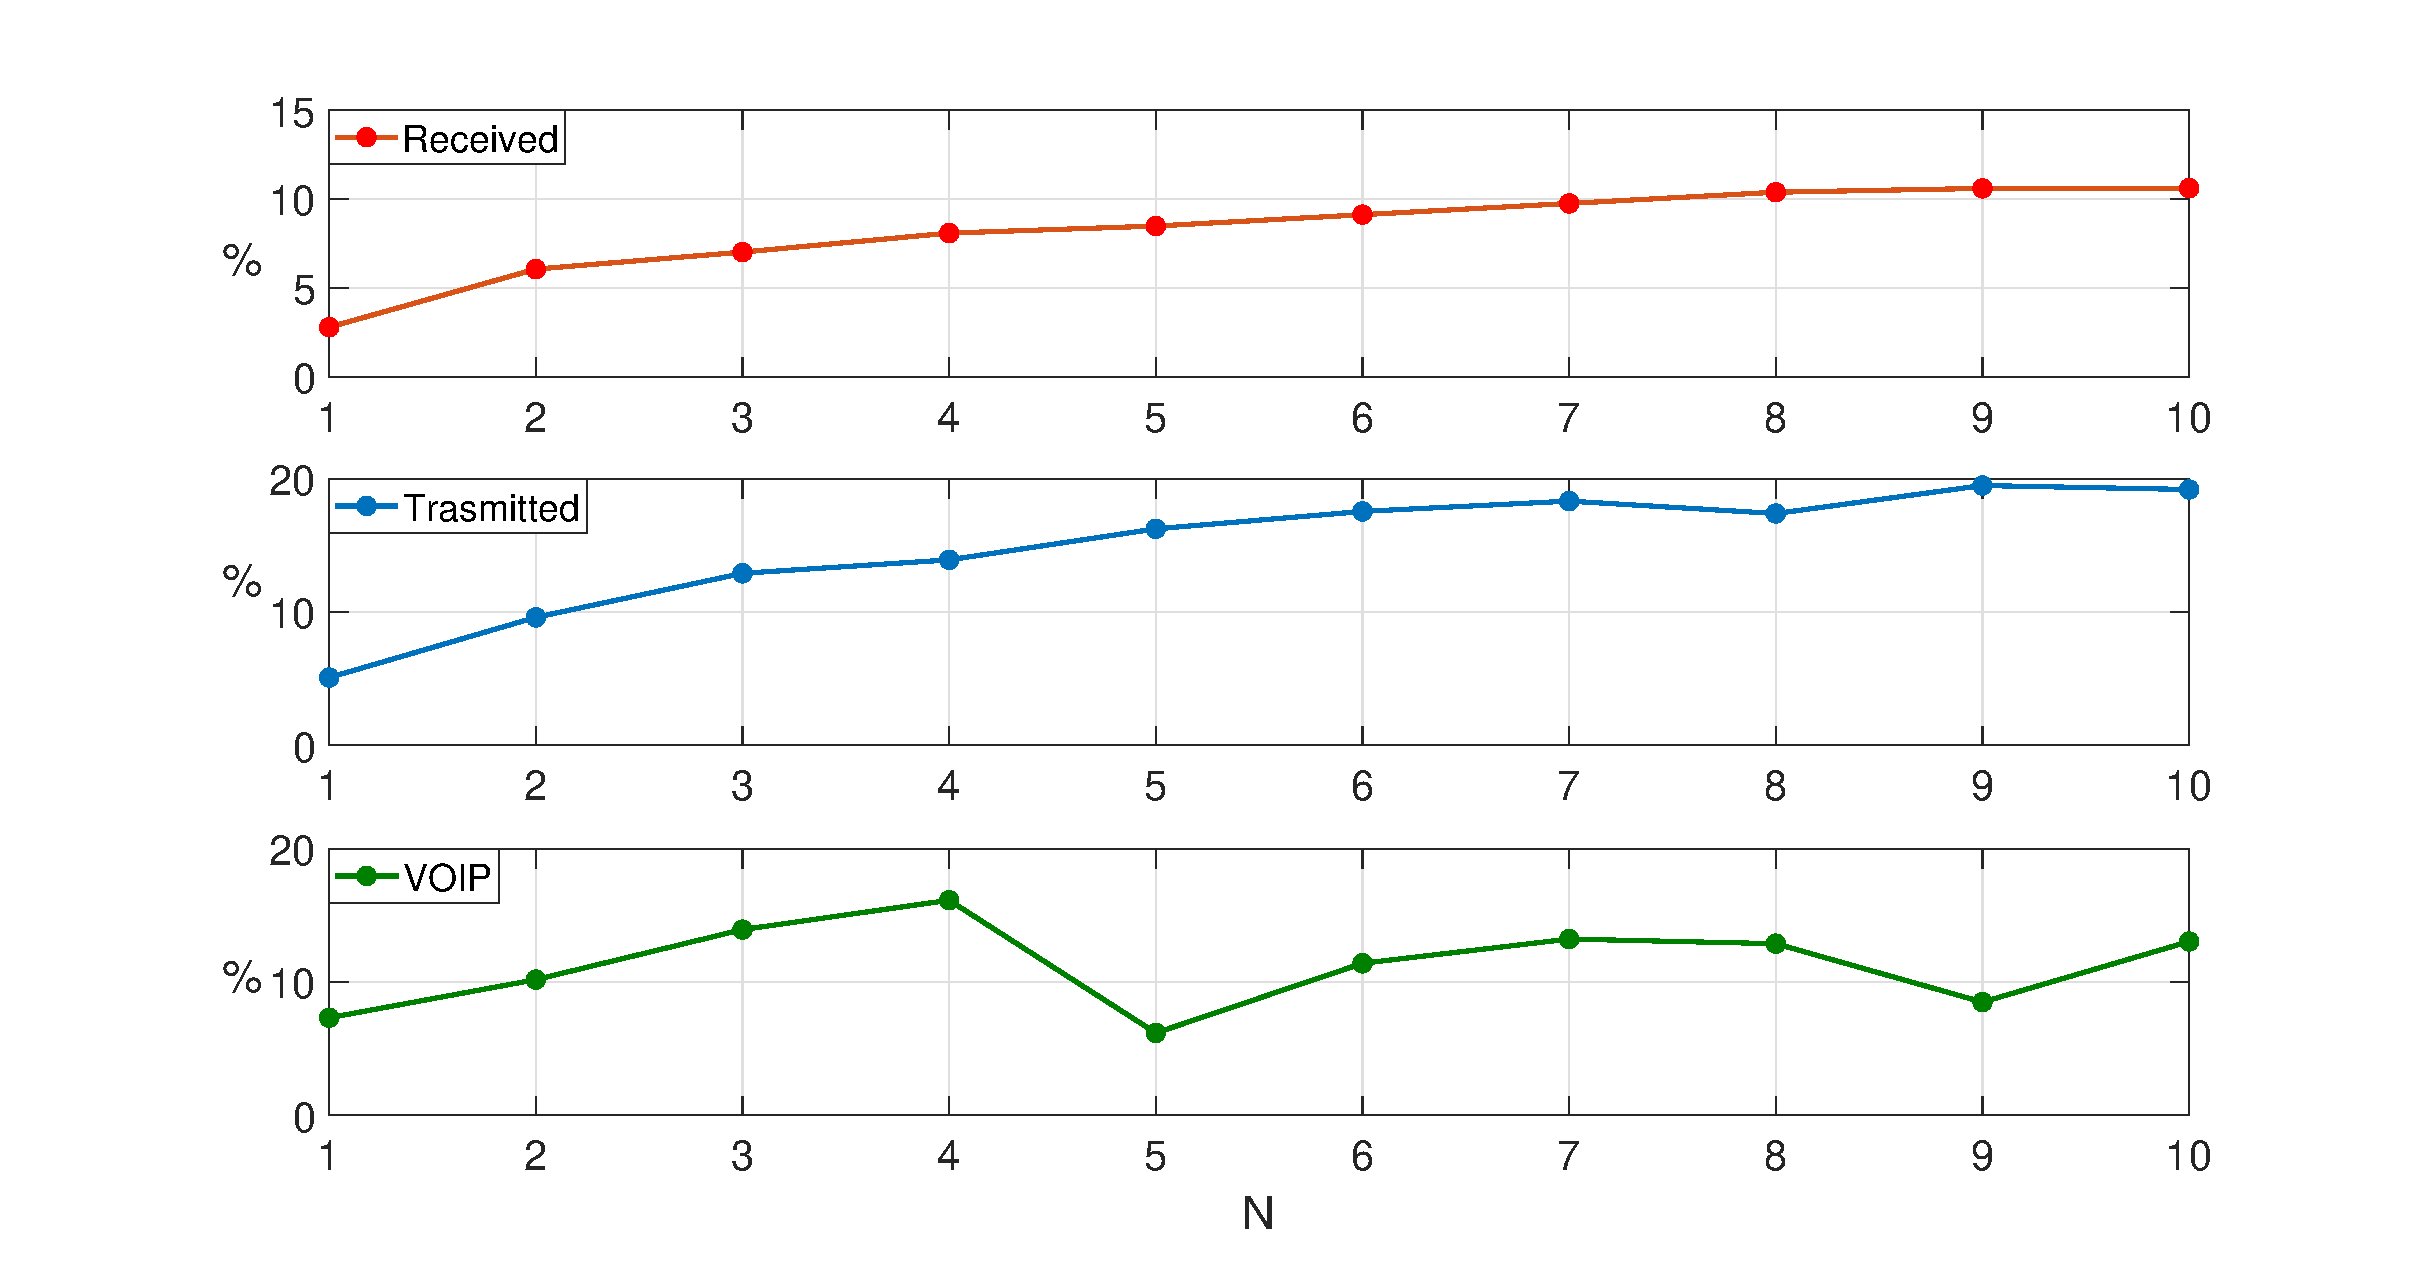
\includegraphics[trim={120 0 120 0}, width=1\linewidth]{figure/Error_PESCARA_DATA.eps}
	\caption{NRMSE of the packets predictive model over a time horizon of $N=10$.}
	\label{fig:{errorPescara}}
\end{figure}
\subsection{Queues predictive model validation}

In this section a comparison of the accuracy of RT and RF predictive models with Artificial Neural Networks will be showed. A neural network is a collection of algorithms that identify underlying relations in a dataset: it consists of groups of connected neurons organized in layers, where the connections between neurons are modeled using weights. The signal produced with this linear composition is then fed into an activation function that is in general nonlinear. The reader is referred to \cite{NNstateOfART} and references therein for more details. A wide number of tools to build Neural Networks have been developed during recent years, e.g. \cite{tensorflow2015,chollet2015keras,openNN} just to mention a few: in this work it is exploited the Deep Learning Toolbox of Matlab to compare predictive models based on NNs with the methodology proposed in this paper, based on ARX combined RTs and RFs. It is considered here just OLD as the learning dataset and a predictive horizon $N=5$.

To identify a RT (resp. RF) based predictive model of the queues it is trained a Regression Tree (resp. Random Forest) for each output and for each time horizon, with a total of $15$ trees (resp. $15$ forests each consisting of $30$ trees). The main parameters used for the identification algorithm (see Section \ref{secSwitchedModeling} and Problem \ref{pbLeastSquareProblem}) are summarized in Table \ref{tab:idPar}.  
\begin{table}[h!]
	\caption{Identification parameters}
	\centering
	\begin{tabular}{l c l c}
		\hline\hline
		Parameters & Value & Parameters & Values\\ 
		\hline
		N          & 5   & $f_{min}$  & -100 \\
		$\delta_y$ & 1   & $f_{max}$  & 100  \\
		$\delta_x$ & 5   & $a_{min}$  & -100  \\
		$\delta_u$ & 0   & $a_{max}$  & 100 \\
		$\delta_d$ & 5   & $b_{min}$  & 0  \\
		$\delta$   & 5   & $b_{max}$  & 10000  \\
		$|\Fij|$   & 30  & Minleaf    & 13\\
		\hline
	\end{tabular}
	\label{tab:idPar}
\end{table}
{In particular, as done with $\delta$ in Equation \eqref{eqIdentifiedModelN}, parameters $\delta_x$ and $\delta_d$ are considered as regressive terms of the state and disturbance that will be only used to grow the trees and the forests, i.e. $\sigma_j(k) = \sigma_j(x(k),\ldots,x(k-\delta_x),\bold{u^-}(k),d(k),\ldots,d(k-\delta_d))$. The regressive terms ($\delta_d$, $\delta_y$, $\delta_x$, $\delta_u$, $\delta$)} and the minimum number of samples for each tree of each forest (MinLeaf) have been chosen, with a trial and error approach, considering that very small regressive horizons and very large values for MinLeaf may lead to inaccurate prediction (as they do not provide sufficient information on the past) but very large regressive horizons and very small values for MinLeaf also lead to inaccurate prediction (as they interpolate very old data that might negatively affect the results and produce overfitting).

Regarding specific parameters used for running NN, and for the sake of a fair comparison, they have been tuned to obtain the best performance: in particular shallow networks of 2 layers are considered since deeper networks did not improve the accuracy and, instead, have the negative effect of increasing the sensitivity of the accuracy with respect to the initial conditions of the weights. Among the many algorithms for optimizing the weights of the neurons, the following will be considered: \textit{Scaled conjugate gradient back-propagation} described in \cite{Moller1990}, which provided the best accuracy with respect to the dataset considered. Regarding the activation functions, both the classical sigmoid function (\textit{LogSig}) and the Hyperbolic tangent sigmoid transfer function (\textit{TanSig}) are used.
\begin{figure}[h!]
	\centering
	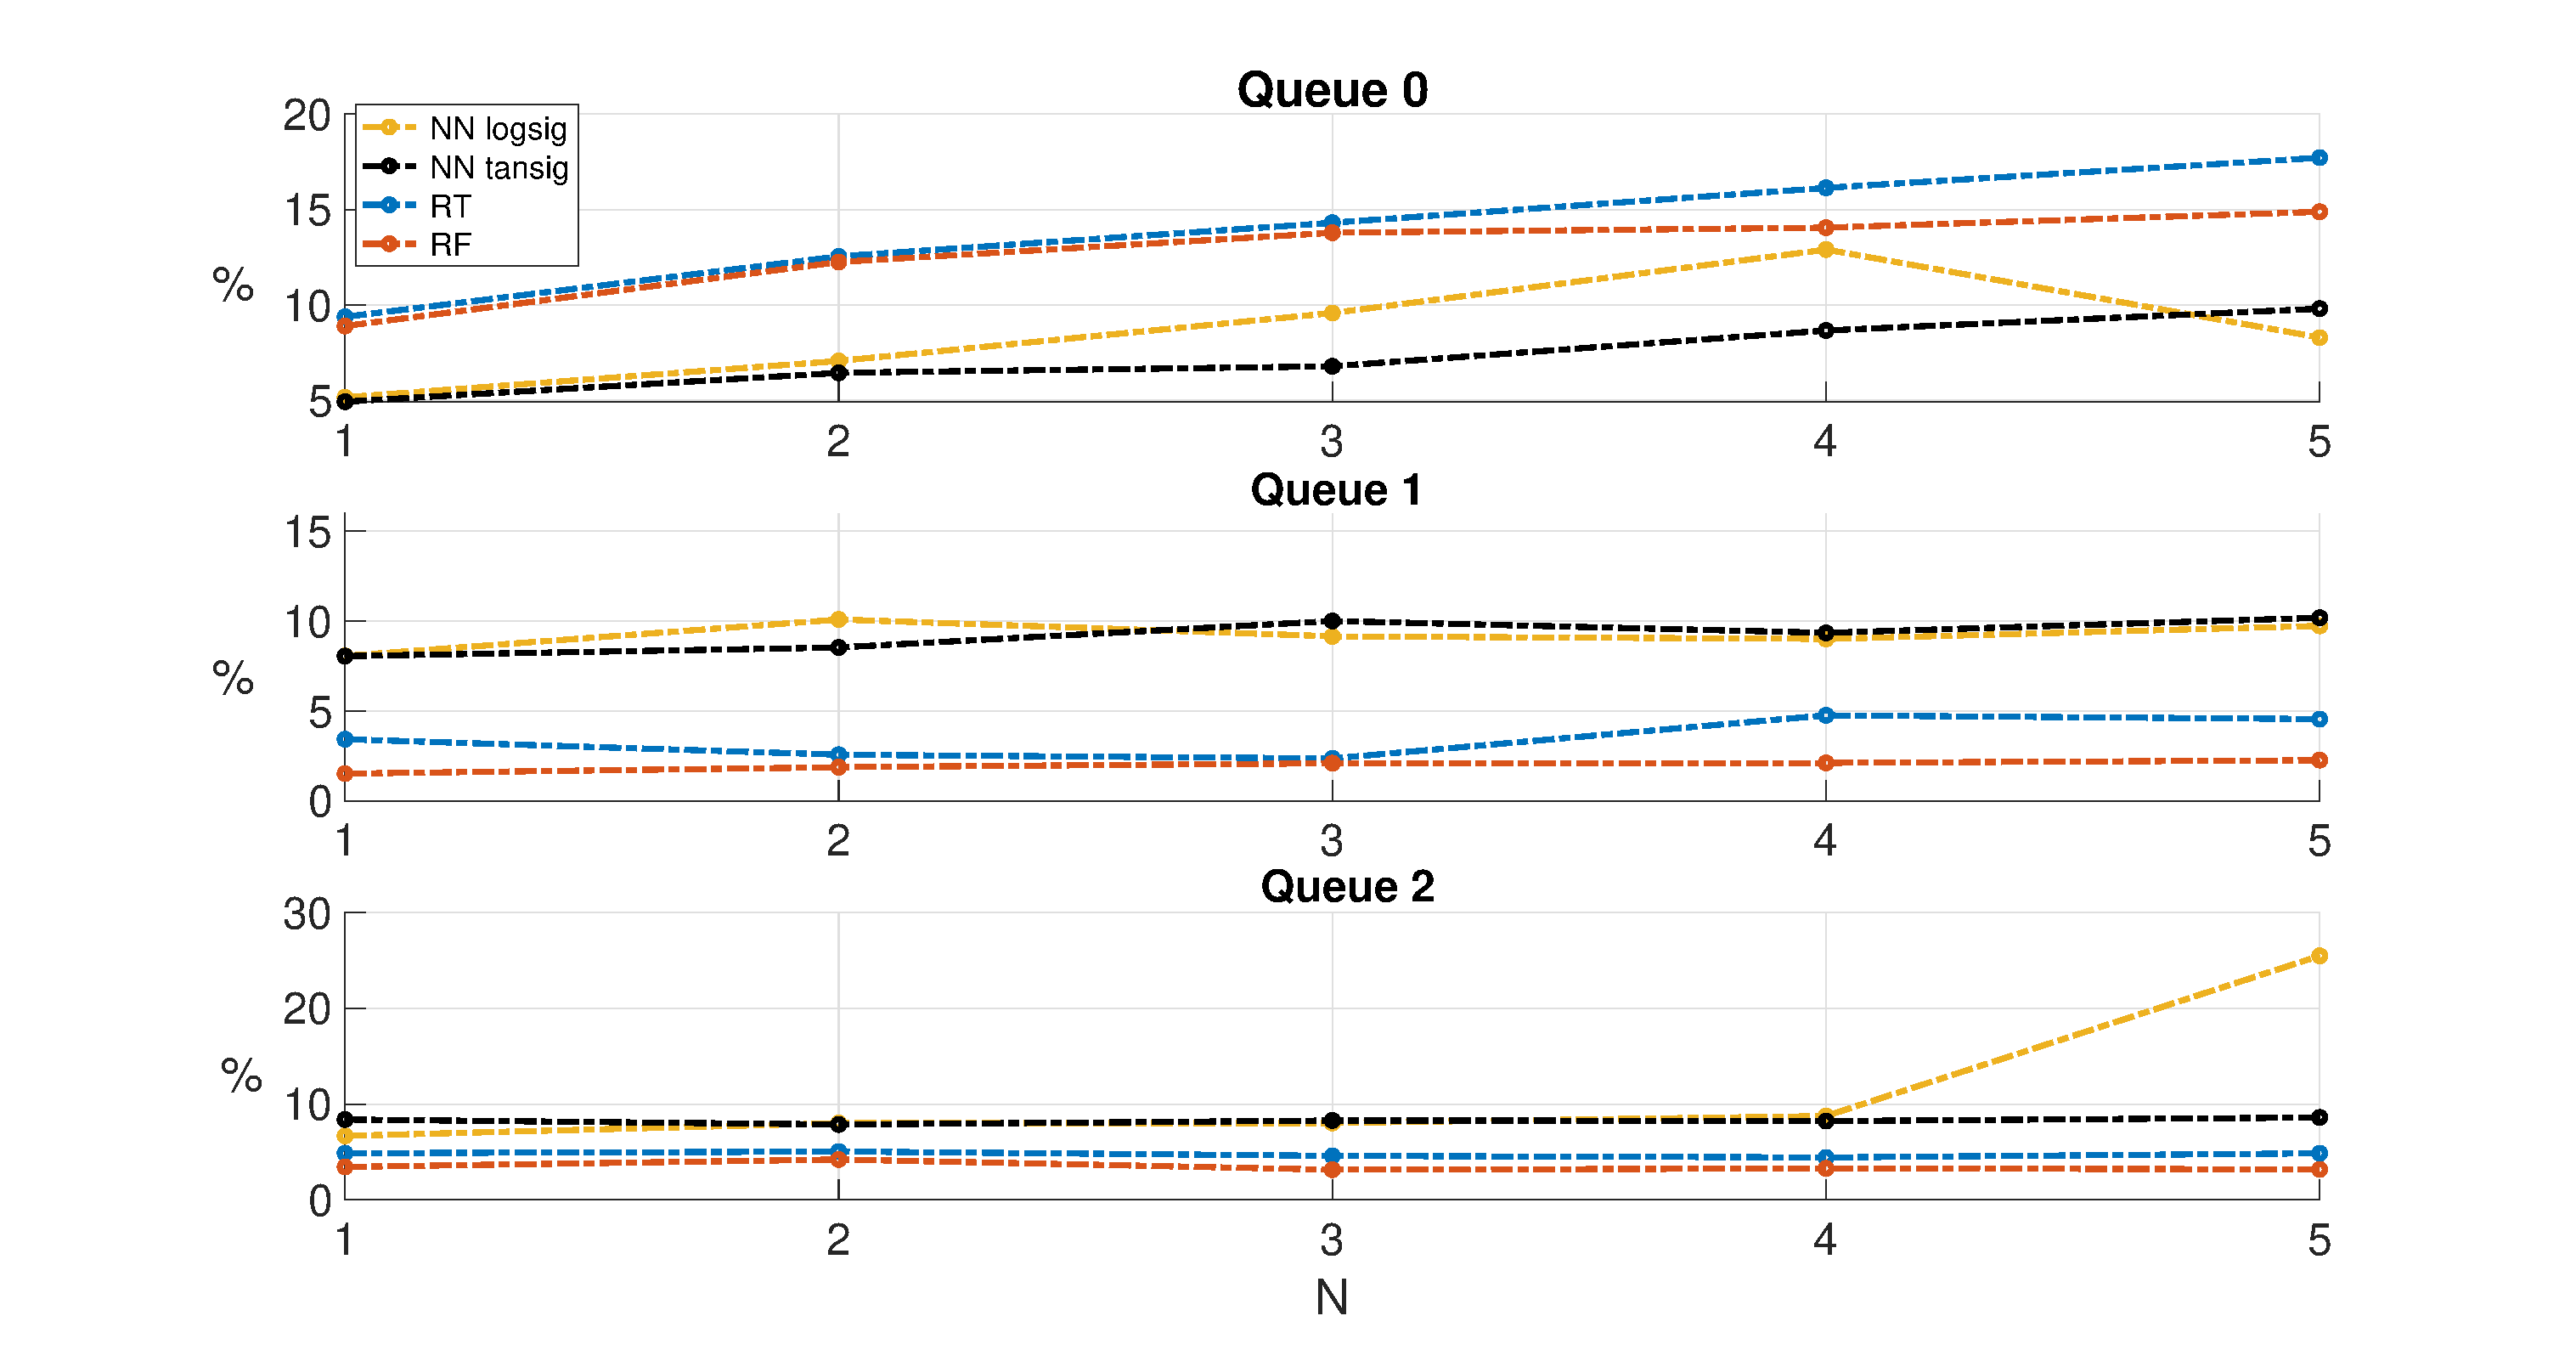
\includegraphics[trim={120 0 120 0},width=0.9\linewidth]{figure/NRMSENNvsRTvsRF.eps}
	\vspace{-0.2cm}
	\caption{NRMSE, up to $N=5$ and for each priority class, for RT (blue), RF (red), NN with sigmoids as activation function (yellow) and NN with hyperbolic tangent as activation function (black).}
	\label{fig:{NRMSE}}
\end{figure}

As a metric of the prediction accuracy in Figure \ref{fig:{NRMSE}} is shown a comparison between the Normalized Root Mean Square Errors (NRMSE) of the different identification approaches for each priority class and over a horizon up to $N=5$. Regarding queue $0$ (Default) NNs perform better than RT and RF, but in queues $1$ (Premium) and $2$ (Gold), characterised by higher priority, RF provides the best performance. Queue $0$ is characterised by a larger NRMSE with all identification techniques: this is due to the fact that, having the lowest priority, it suffers more packet losses and this can negatively affect the prediction accuracy. The validation emphasizes that RTs, even thought very simple and fast to compute, are often affected by overfitting and variance issues, i.e. small variations of the training data result in large variations of the tree structure and, consequently, of the predictions. Regarding NNs, they provide a less accurate model in 2 cases over 3. Indeed, by analyzing the dataset distribution, it is possible to notice a peculiar regular grid pattern that can be very well approximated by hyper-rectangles: since RTs and RFs base their prediction on hyper-rectangular dataset partitions, the better performance with respect to NNs is reasonable. For queue 0, even thought NNs perform better, it is important to remark that their predictive model is based on nonlinear functions: this makes the derived model impractical for real-time control as the corresponding MPC formulation turns into a nonlinear optimization problem, for which there is no approach that can guarantee neither a global optimal solution nor a reasonable computation time. In addition to this, even obtaining a closed mathematical form of the predictive function of a Neural Network starting from neurons and weights is not always an easy task, because of the highly nonlinear interconnections between the different layers. For all these reasons it will be only used, from now on, RF-based models which provide the best choice both from the accuracy and the computational complexity points of view. In the following it is illustrated the effect of iterative dataset updates in the prediction accuracy, both with and without prediction of the future disturbances.
\begin{figure}[th!]
	\centering
	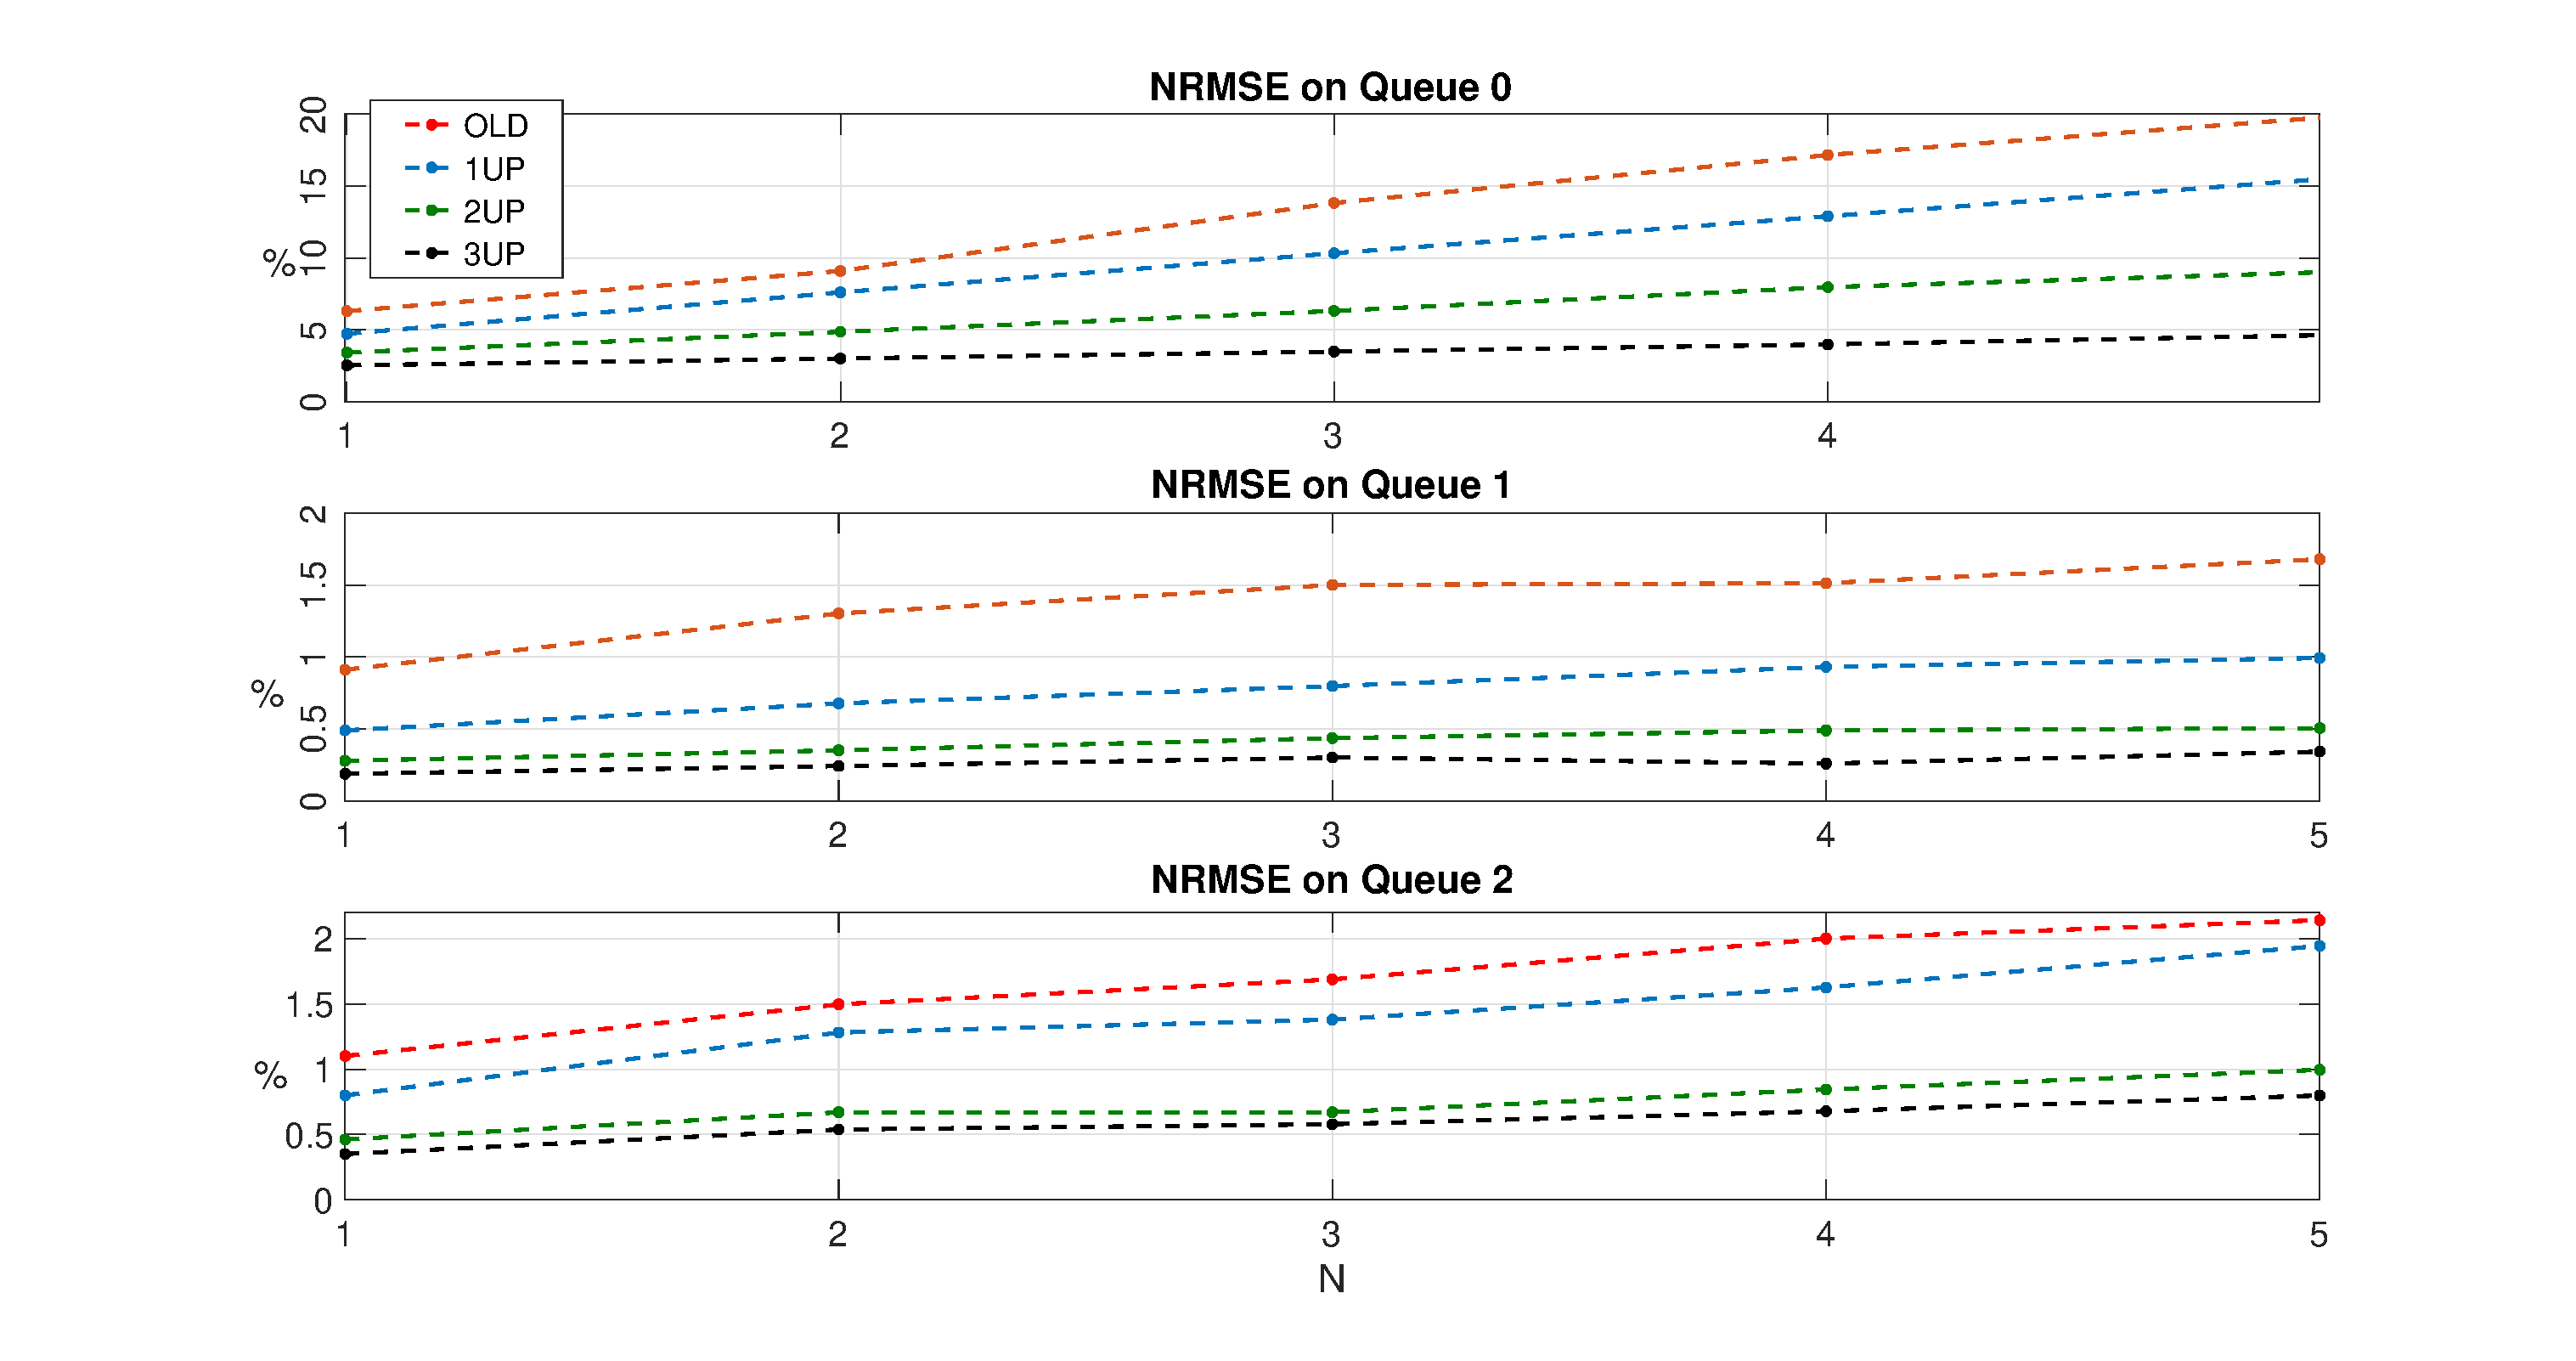
\includegraphics[trim={120 0 120 0}, width=0.9\linewidth]{figure/Error_State.eps}
	\caption{NRMSE of the queues output predictive model over a time horizon of $N=5$, without prediction of the future disturbances}
	\label{fig:{stateNRMSE}}
\end{figure}
\begin{figure}[th!]
	\centering
	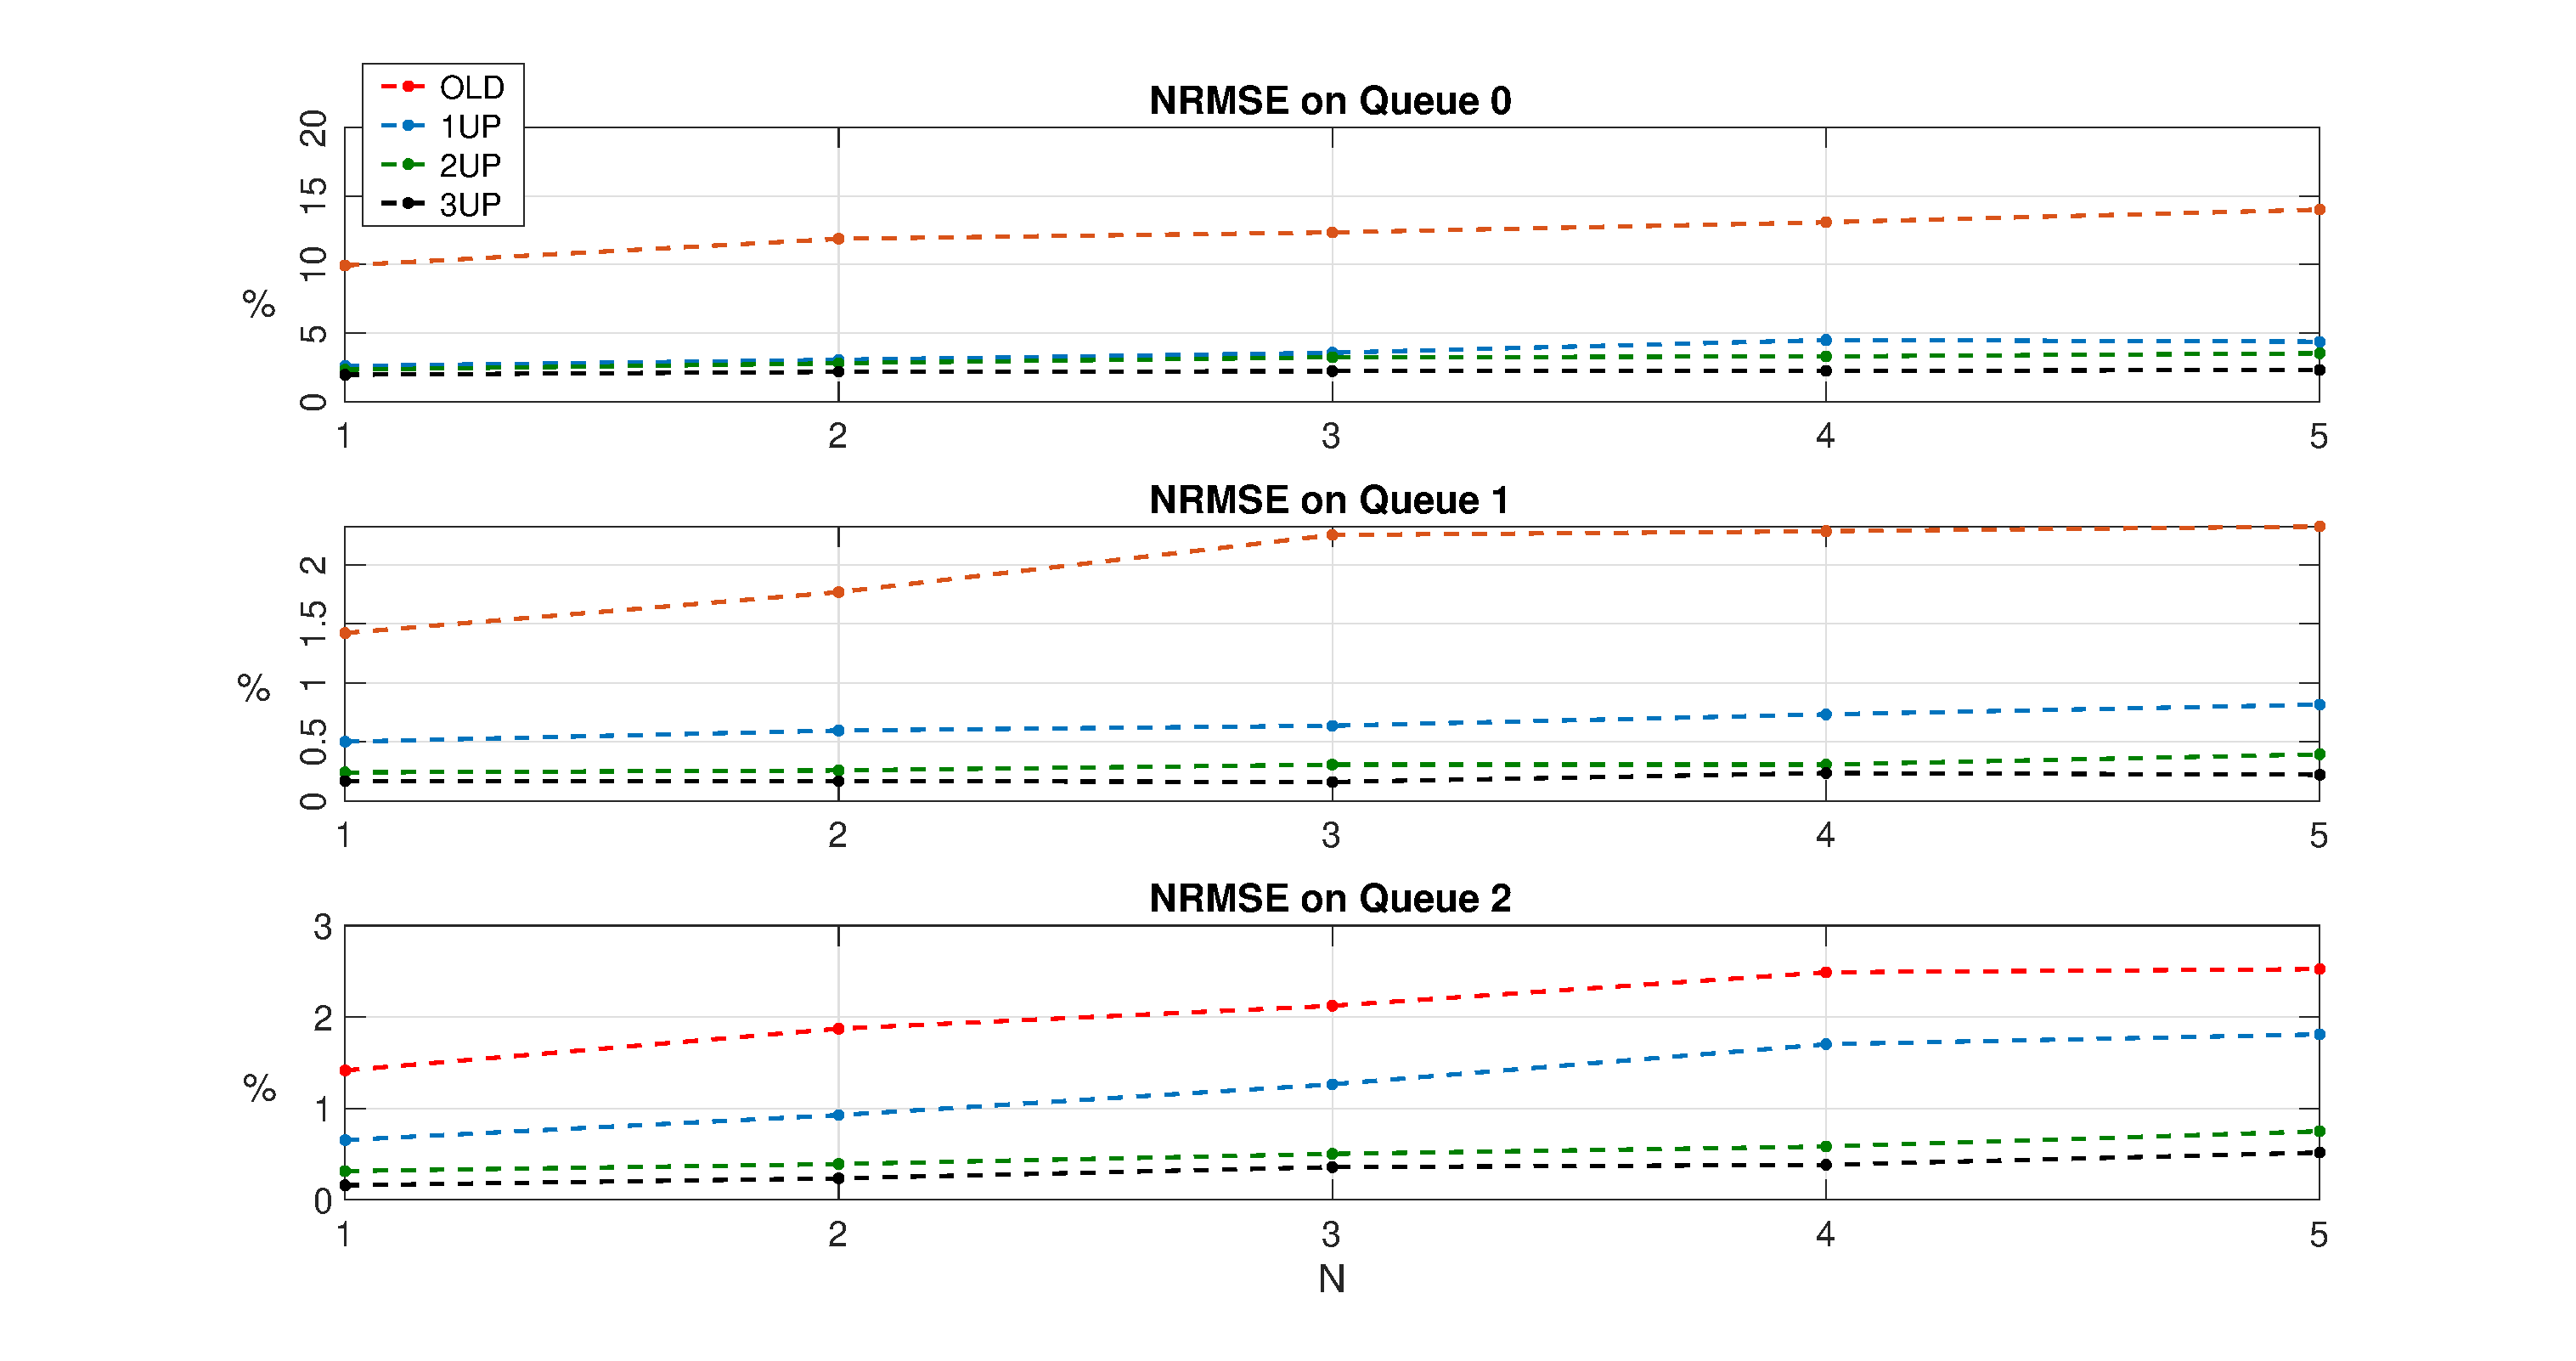
\includegraphics[trim={120 0 120 0}, width=0.9\linewidth]{figure/Error_State_ddM4.eps}
	\caption{NRMSE of the queues output predictive model over a time horizon of $N=5$, with prediction of the 4-steps future disturbances}
	\label{fig:{stateNRMSEddM4}}
\end{figure}

Figure \ref{fig:{stateNRMSE}} and Figure \ref{fig:{stateNRMSEddM4}} plot the NRMSEs respectively without and with prediction of the future disturbances. The assumption of future disturbance forecast, as expected, provides much better prediction accuracy. The positive effect of updated data sets is also clear, providing accuracy improvements up to $50 \%$: as will be also discussed in the next section, the most relevant prediction accuracy improvement takes place moving from OLD to 1UP or from 1UP to 2UP, while the 3UP model does not improve much.

\begin{remark}
In the simulations shown in this work, data are generated without major modifications of the traffic daily pattern: for this reason enriching the data set converges to a saturation of the model accuracy, as discussed above. Nevertheless, the capability of the proposed methodology to iteratively learn from new data is fundamental as, in real life, changes in the traffic patterns do occur, and model updates are necessary to maintain the model accuracy and the control performance. 
\end{remark}

%====================================================================================================

\subsection{Control performance}

In this section a control loop is setup, where the (Mininet) network emulator and the (Ryu) controller run in two different computers, and synchronize/exchange data using a shared file. Namely, the SW controller module is ready to be directly used on a real SDN-based network, with just some minor modifications in the data exchange with the switch devices. The controller implements MPC using the predictive models validated in the previous sections: at each time step, it solves Problem \ref{pbMPC} and optimally updates the bandwidth of the different queues. The cost matrices $Q$ and $R$ of Problem \ref{pbMPC} respectively weight the output $y(k)$ of the system (i.e. the packet transmission rate for each queue) and the control input $u(k)$ (i.e. the bandwidth assigned to each queue). Since $R$ is required to be positive definite but it makes no sense assigning a penalty to the choice of $u(k)$, the choice has been $R=10^{-5} \cdot \mathbb I$, where the identity matrix $\mathbb I$ multiplies a very small value. Matrix $Q = diag(1,10^4,10)$ has been assigned as a diagonal matrix, where the choice of the different diagonal components is related to the priority level of each queue. The remaining constraints of Problem \ref{pbMPC} are reported in Table \ref{tab:contPar}.
%The parameters used in the constraints described in Problem \ref{pbMPC} are reported in Table \ref{tab:contPar} and the weights matrices considered in the optimisation cost are: $Q=diag([1,1000,10])$ and $R=10^{-5} \mathbb{I}_3$.
\begin{table}[h!]
	\caption{Constraints in Problem \ref{pbMPC}}
	\centering
	\begin{tabular}{l c l c}
		\hline\hline
		Parameters                                & Value               & Parameters                 & Values       \\ 
		\hline
		$\Delta u_1^\mathrm{min}$     & 1                   & $\Delta u_1^\mathrm{max}$  & 30           \\
		$\Delta u_2^\mathrm{min}$     & 20                  & $\Delta u_2^\mathrm{max}$  & 30           \\
		$\Delta u_3^\mathrm{min}$     & 20                  & $\Delta u_3^\mathrm{max}$  & 20           \\
		$u_1^\mathrm{min} $             & 10                  & $u_1^\mathrm{max} $        & 45           \\
		$u_2^\mathrm{min} $            & 55                  & $u_2^\mathrm{max} $        & 80           \\
		$u_3^\mathrm{min} $            & 80                  & $u_3^\mathrm{max} $        & 100          \\
		
		\hline
	\end{tabular}
	\label{tab:contPar}
\end{table}
In what follows it is validated the control performance both without and with prediction of the future disturbances. The values of $x_{\mathrm{ref},j}$ in the optimization problem represent the reference values chosen for tracking system output: indeed, as the objective is to minimize packet losses, it is minimized the difference between the packets received by the hosts $d(k)$ and those transmitted by the queues $y(k)$ over the horizon $N$. In case there are no prediction of future disturbances, $x_{\mathrm{ref},j}=x_{\mathrm{ref}}=d(k)$ will be equal to the current disturbance  measurement and constant over all the predictive horizon; if instead there is a prediction of future disturbances, $x_{\mathrm{ref},j}$ will be equal to such forecast. In this section are compared only models OLD, 1UP and 2UP, since model 3UP does not provide any substantial improvement. 

 \begin{figure}[h!]
	\centering
	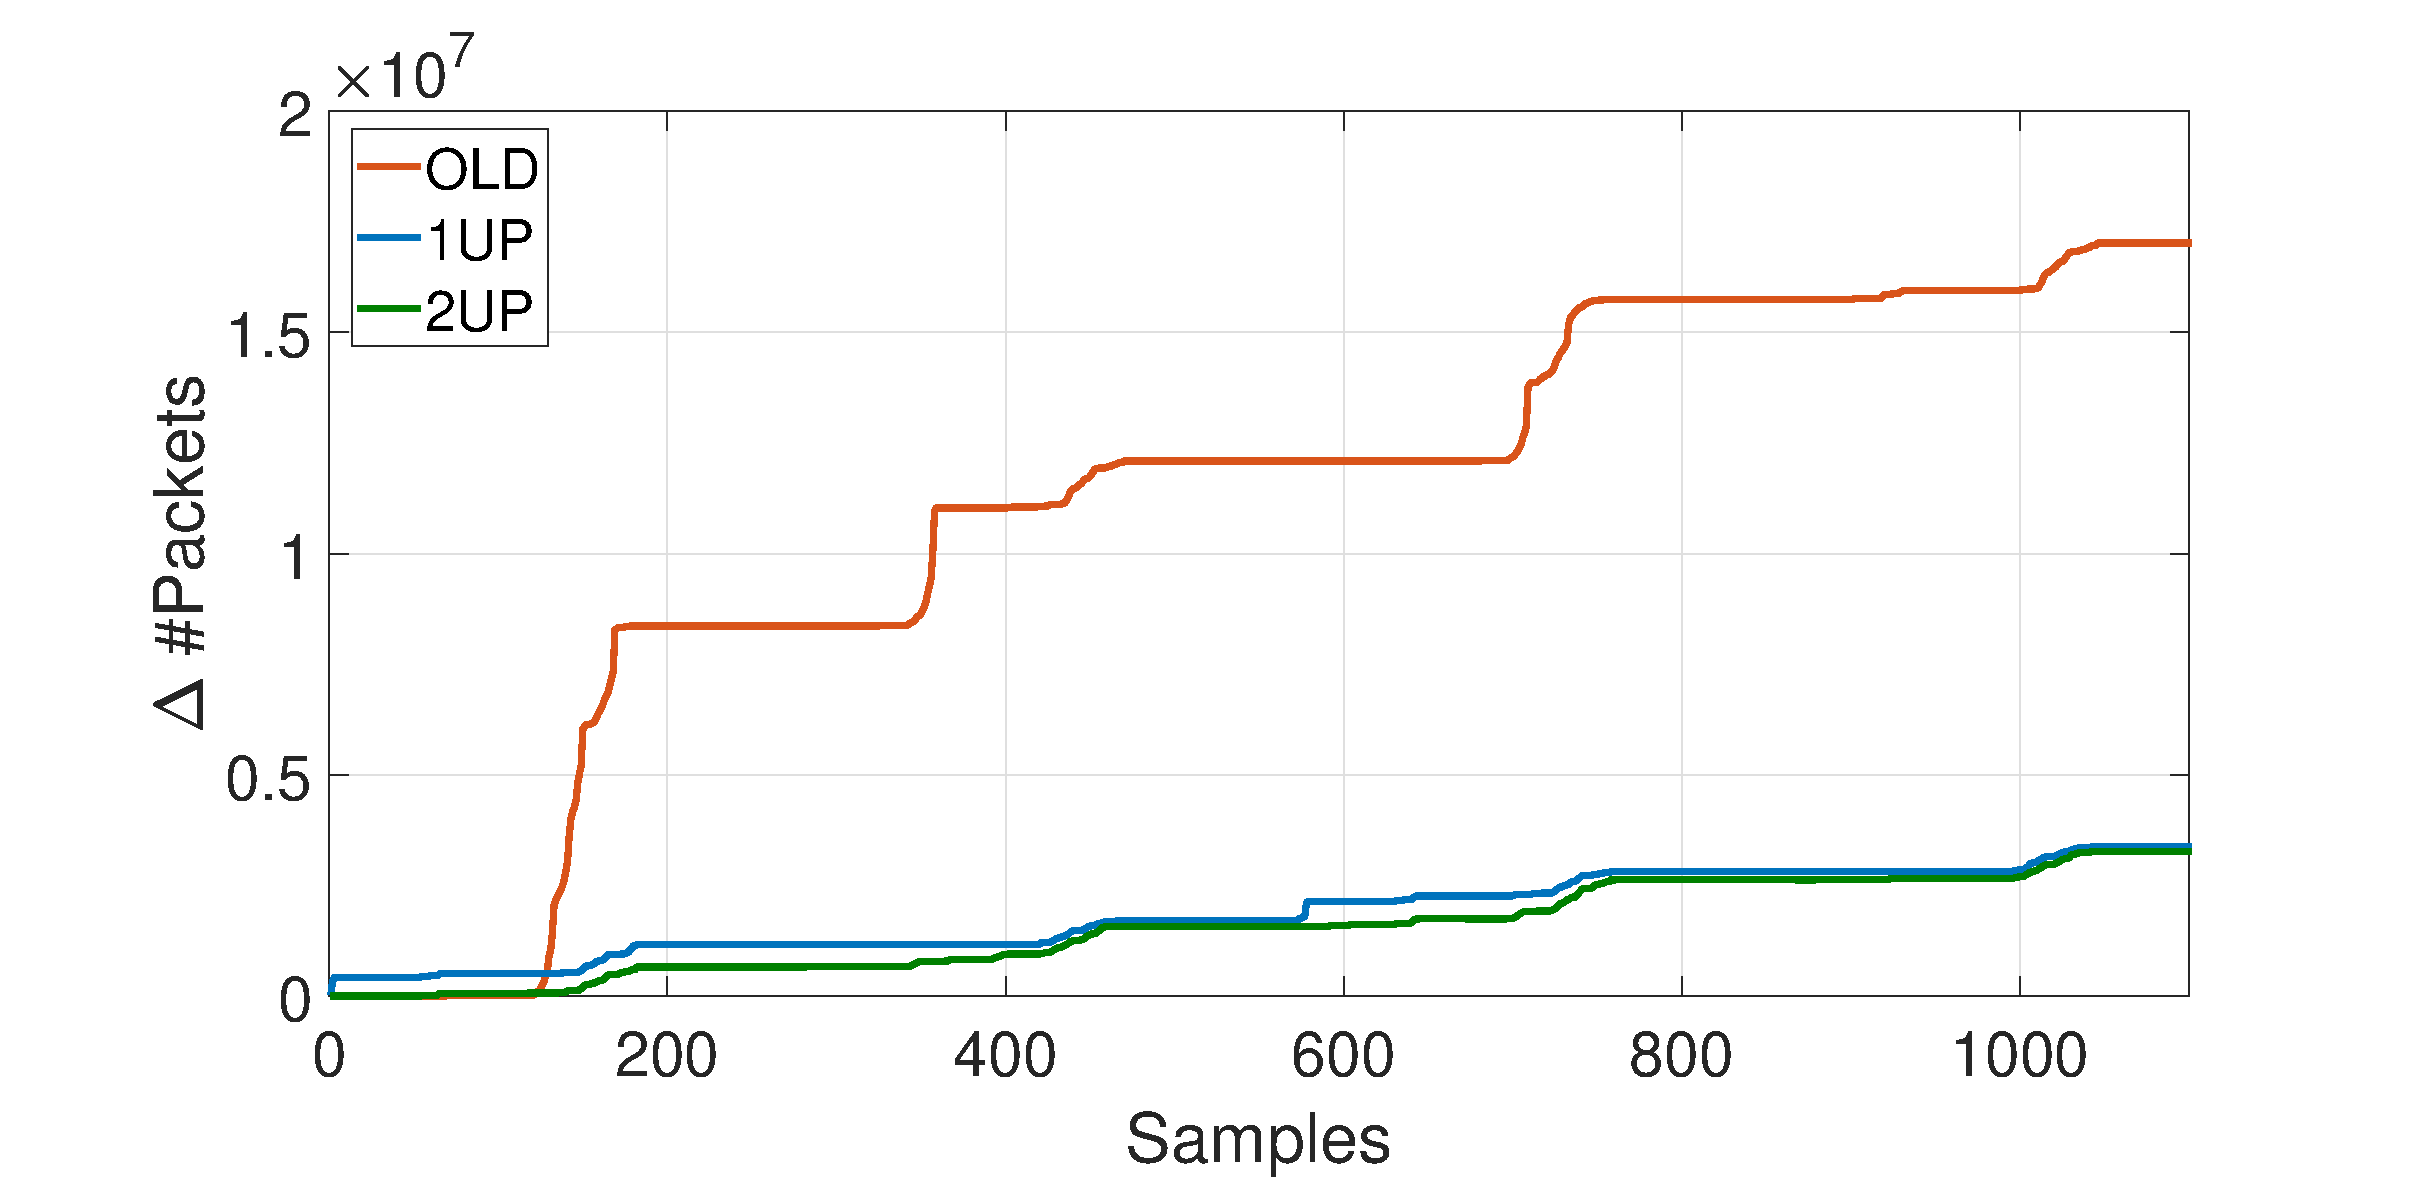
\includegraphics[trim={120 0 120 0}, width=0.9\linewidth]{figure/cumPL1.eps}
	\caption{Cumulative Packet Losses without prediction of the future disturbance.}
	\label{fig:{MPC1}}
\end{figure}
\begin{figure}[h!]
	\centering
	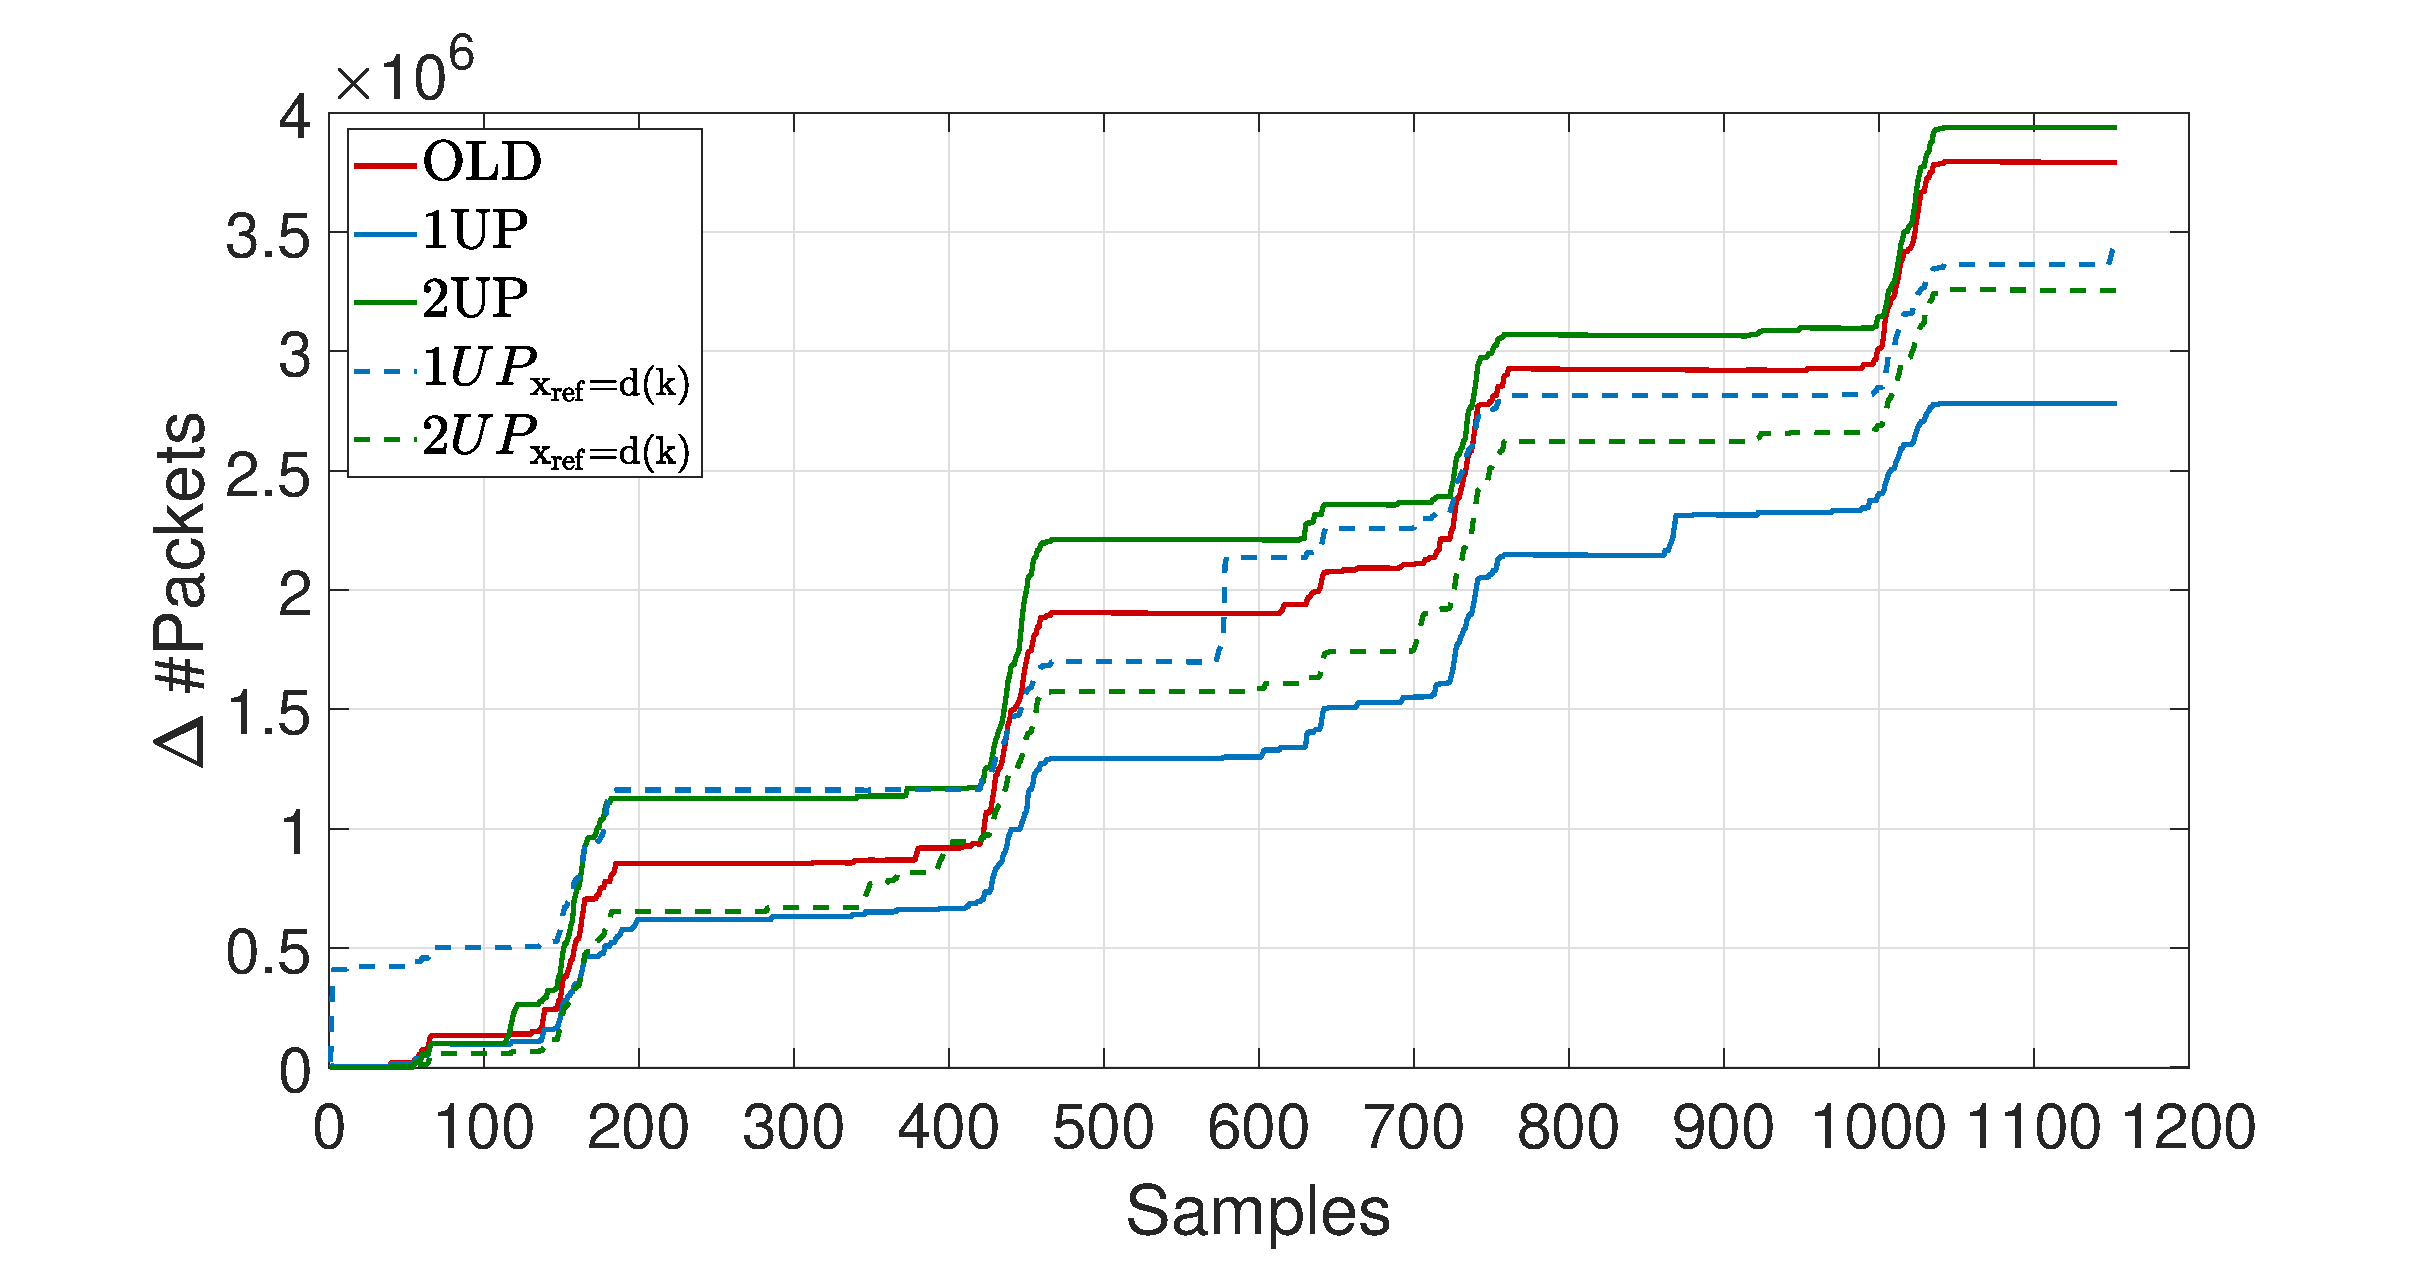
\includegraphics[trim={120 0 120 0},width=0.85\linewidth]{figure/cumPL_Total.eps}
	\caption{Comparison between Cumulative Packet Losses with (solid lines)  and without (dashed lines) prediction of the future disturbance.}
	\label{fig:{MPC2}}
\end{figure}
 Figures \ref{fig:{MPC1}} and \ref{fig:{MPC2}} plot the cumulative packet losses respectively without and with prediction of the future disturbances. The packet loss rate when the control is performed exploiting the OLD model and without disturbance forecast is around $123\%$ larger than all other cases (and, of course, incomparably smaller than the static control case \cite{Notiziario}). It is also clear from the plots that 1UP and 2UP without disturbance forecast and OLD, 1UP and 2UP with disturbance forecast provide very similar performance. Authors' interpretation is that OLD models without disturbance forecast have not enough information to provide good accuracy, but they can be easily improved either with a data set update (which however requires $10$ days for 1UP and $20$ days for 2UP of additional data) or using a predictive disturbance model.

\begin{figure}[h!]
\centering
\subfigure[a][]{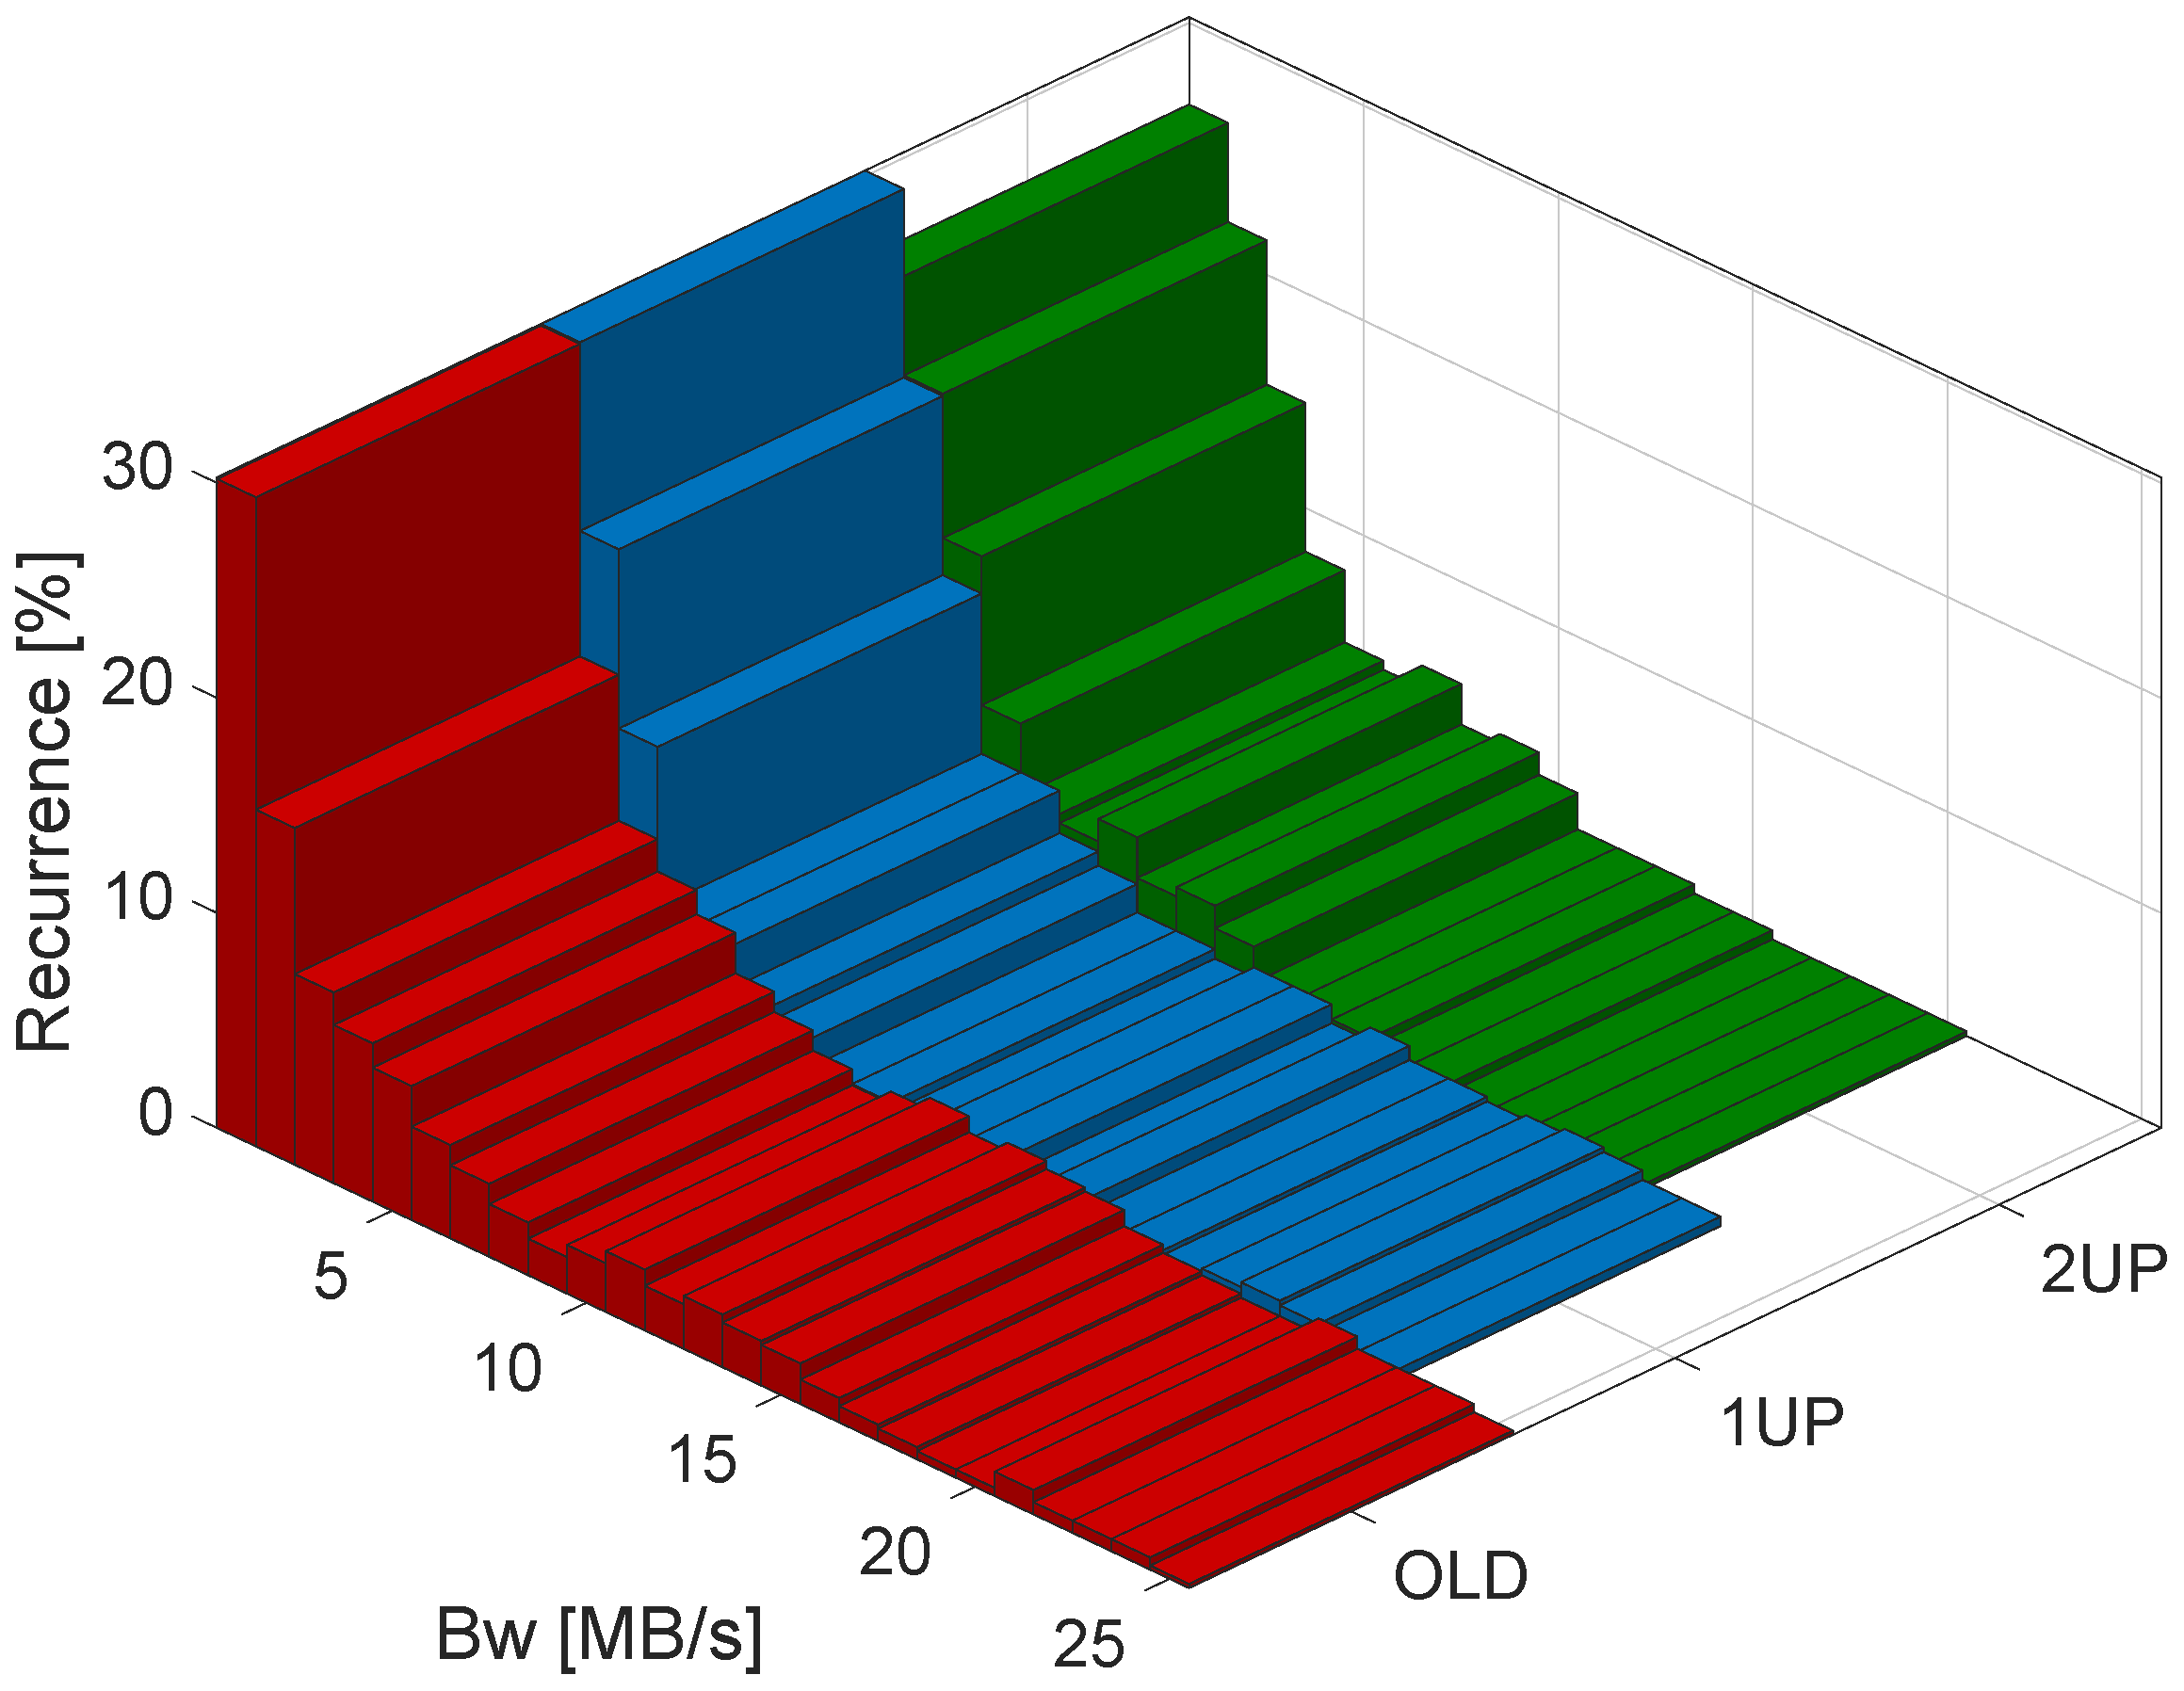
\includegraphics[width=0.7\linewidth]{figure/BW_NoPred.eps}}
\subfigure[b][]{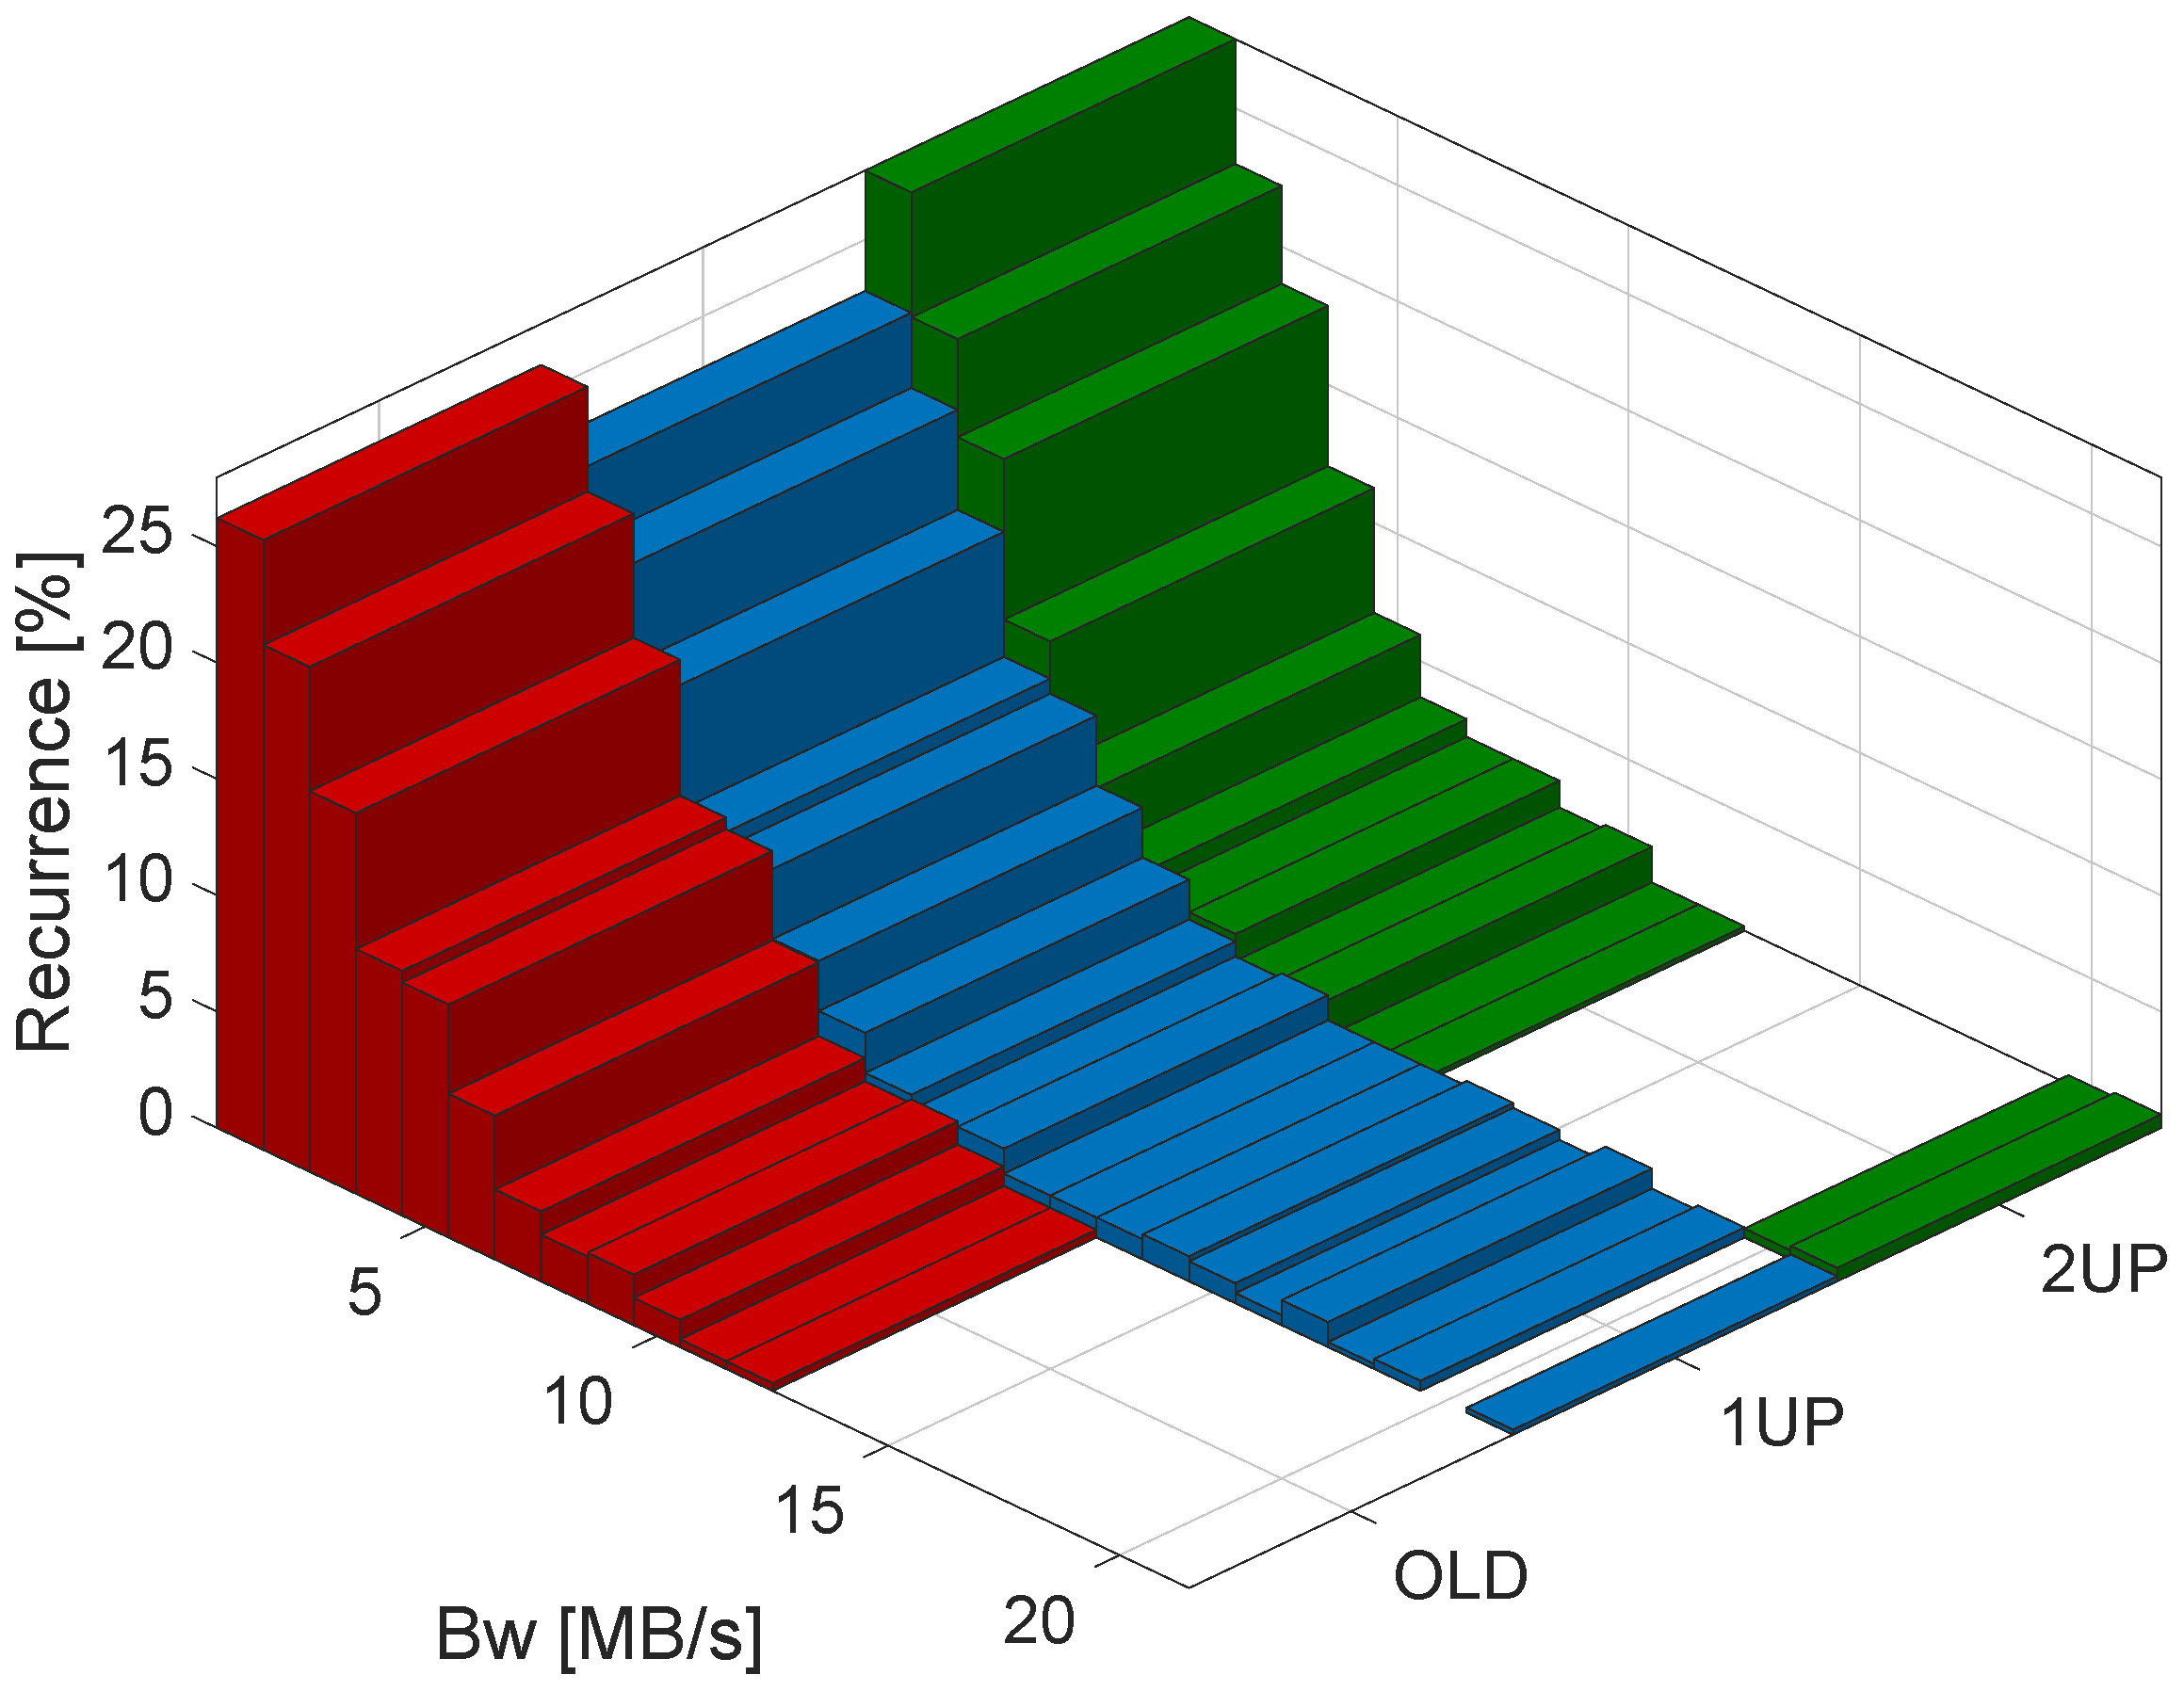
\includegraphics[width=0.7\linewidth]{figure/BW_Pred.eps}}
\caption{Bandwidth saving comparison without (a) and with (b) prediction of the future disturbances.}
\label{fig:BW}
\end{figure}

Figure \ref{fig:BW} illustrates the bandwidth savings showing the recurrence of the different bandwidth usage during the simulations, respectively without and with prediction of the future disturbances. Without disturbance forecast it is exploited up to $25MB/s$ using the OLD model, while it is exploited at most $22MB/s$ and $21MB/s$ respectively for models 1UP and 2UP. Using disturbance forecast, as expected, even less bandwidth is exploited.

\begin{figure}[h!]
\centering
\includegraphics[trim={120 0 120 0},width=0.9\linewidth]{figure/MPCfinal.eps}
\caption{Static controller up to the $400th$ sample, then MPC controller.}
\label{fig:{MPC}}
\end{figure}
\begin{figure}[h!]
	\centering
	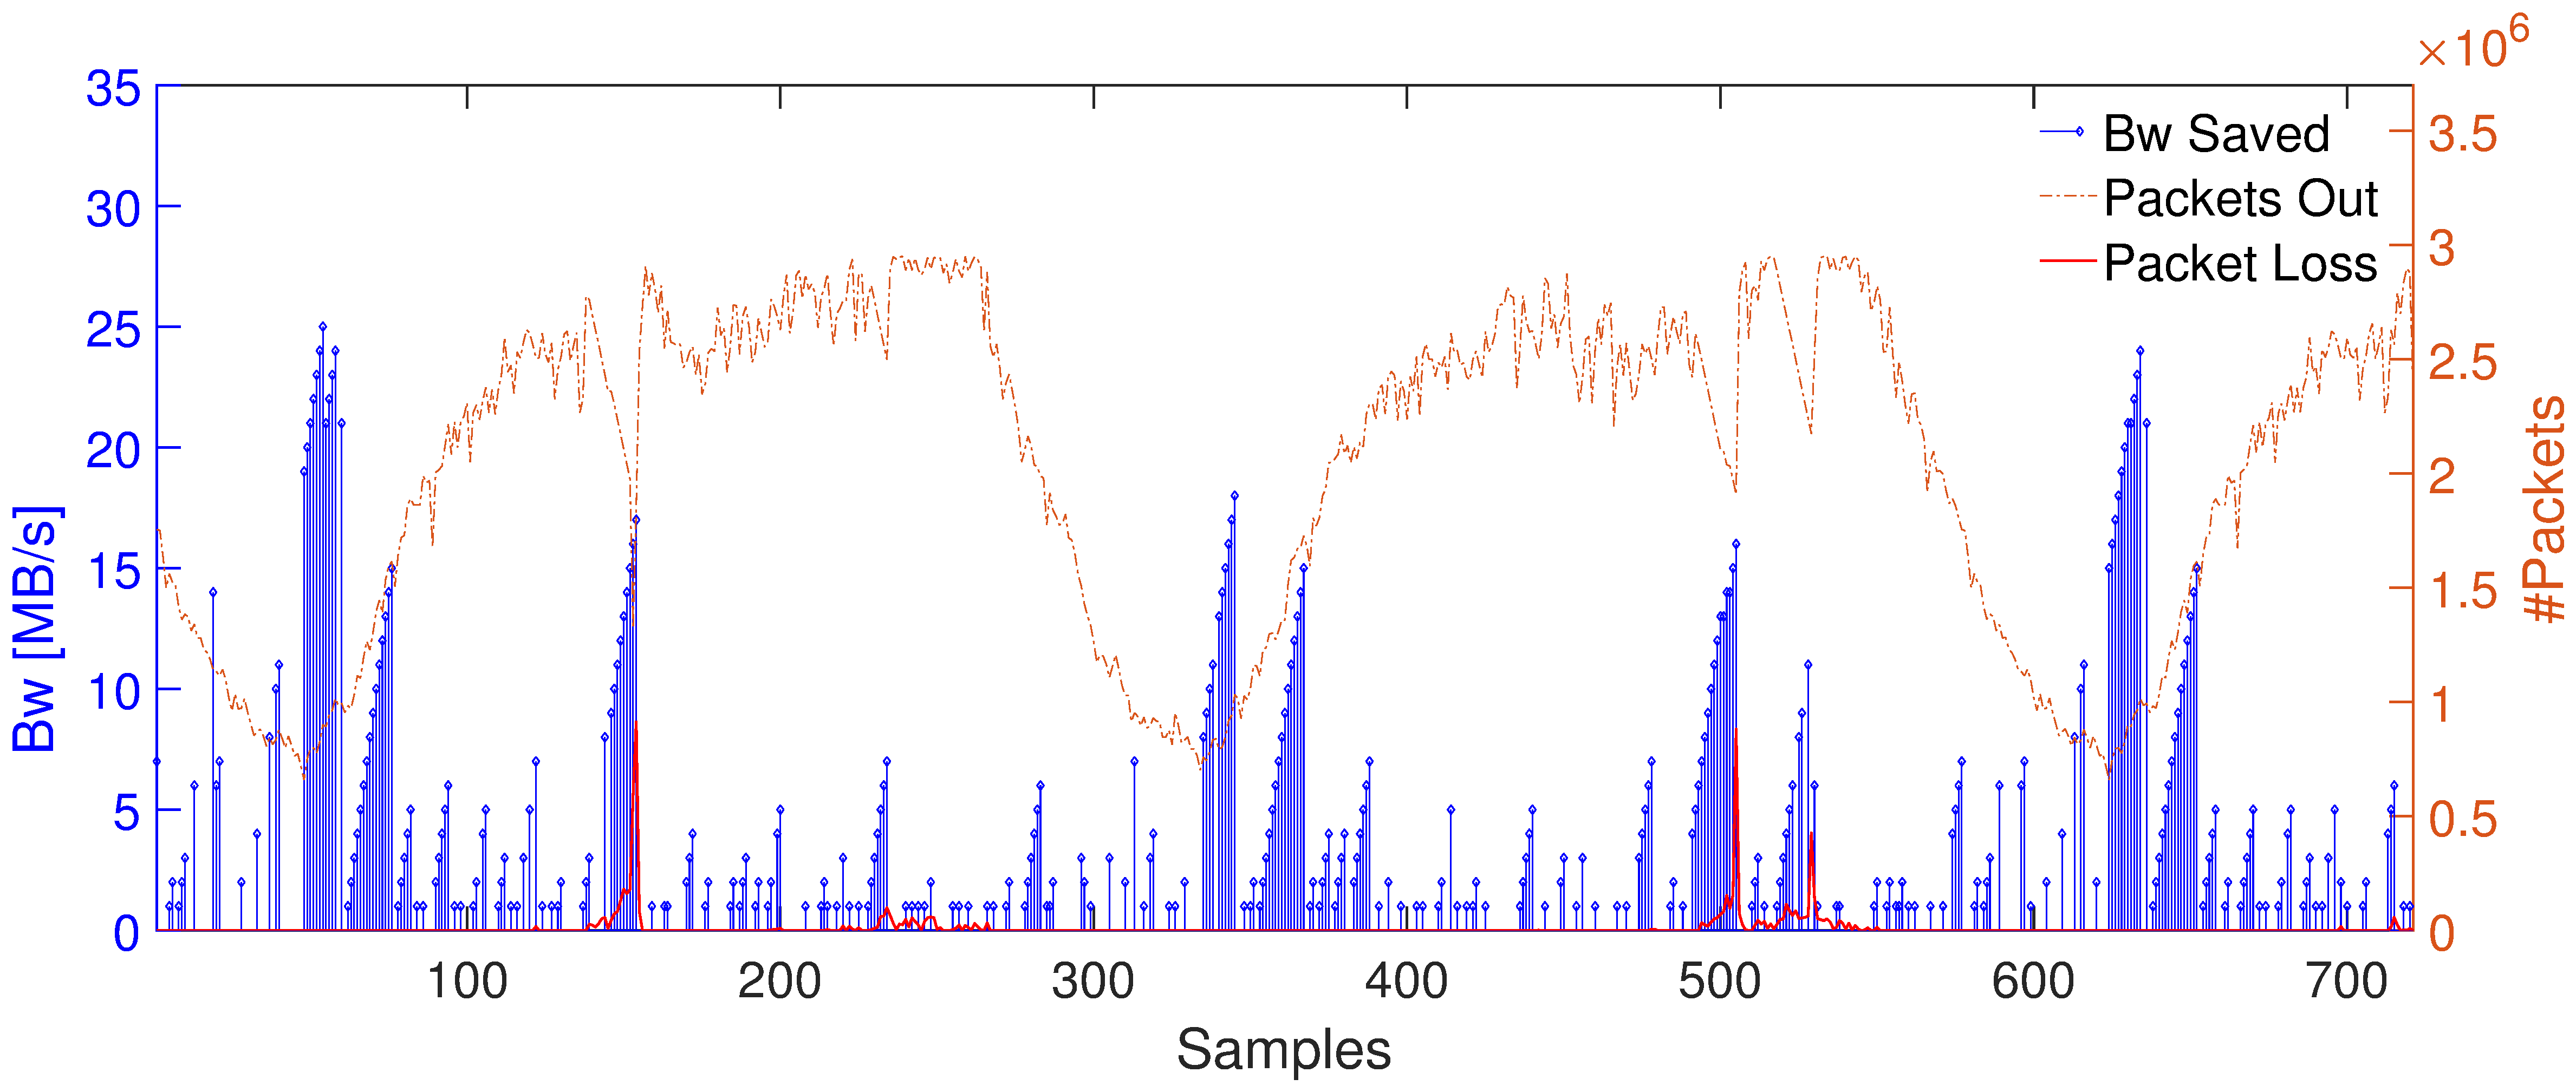
\includegraphics[trim={120 0 120 0},width=1\linewidth]{figure/Banda.eps}
	\vspace{-0.2cm}
	\caption{MPC controller: packets sent from the queues (orange), packets lost (red), bandwidth saving (blue).}
	\vspace{-0.5cm}
	\label{fig:{BWsave}}
\end{figure}


In conclusion to this section, it will be shown the gap between priority queueing control performance of MPC, obtained solving Problem \ref{pbMPC} and based on the proposed RF predictive model, with the static control policy adopted by service provider networks in \cite{Notiziario}. Figure \ref{fig:{MPC}} highlights the dramatic improvement of MPC with respect to static control: the red line shows the incoming traffic, the blue line shows the sum of the packets sent from the queues, and their difference represents packet losses. Until the $400th$ sample static control has been implemented as in \cite{Notiziario}, generating many packet losses due to queues saturation. From that sample to the end of the experimentation MPC is implemented using RF-based model, and the packet loss is drastically reduced: quantitatively, after $700$ sampling periods the cumulative number of dropped packets with the static policy is about $5.5\cdot10^8$ versus $6.6\cdot10^6$ with MPC, with a decrease of $5.434\cdot10^8$ lost packets ($-88 \%$).
%Figure \ref{fig:{BWsave}} shows the amount of bandwidth that our method leaves unused at each time sample (blue line): during the simulation period we were able to save an average $3 MB/s$ with respect to static control, with peaks of more than $20 MB/s$, that can be of course allocated to improve the quality of other services.
Even thought the improvement of MPC with respect to static control is not surprising, much better performance can be obtained in real networks just collecting historical data and applying a controller that can be directly implemented using the accurate models of the proposed identification algorithms and Quadratic Programming standard solvers.

%====================================================================================================
%====================================================================================================